%%%%%%%%%%%%%%%%%%%%%%%%%%%%%%%%%%%%%%%%%%%%%%%%%%%%%%%%%%%%%%%%%%%%
%% I, the copyright holder of this work, release this work into the
%% public domain. This applies worldwide. In some countries this may
%% not be legally possible; if so: I grant anyone the right to use
%% this work for any purpose, without any conditions, unless such
%% conditions are required by law.
%%%%%%%%%%%%%%%%%%%%%%%%%%%%%%%%%%%%%%%%%%%%%%%%%%%%%%%%%%%%%%%%%%%%

\documentclass[
  digital, %% The `digital` option enables the default options for the
           %% digital version of a document. Replace with `printed`
           %% to enable the default options for the printed version
           %% of a document.
%%  color,   %% Uncomment these lines (by removing the %% at the
%%           %% beginning) to use color in the printed version of your
%%           %% document
  oneside, %% The `oneside` option enables one-sided typesetting,
           %% which is preferred if you are only going to submit a
           %% digital version of your thesis. Replace with `twoside`
           %% for double-sided typesetting if you are planning to
           %% also print your thesis. For double-sided typesetting,
           %% use at least 120 g/m² paper to prevent show-through.
  lof,     %% The `lof` option prints the List of Figures. Replace
           %% with `nolof` to hide the List of Figures.
  lot,     %% The `lot` option prints the List of Tables. Replace
           %% with `nolot` to hide the List of Tables.
]{fithesis4}
%% The following section sets up the locales used in the thesis.
\usepackage[resetfonts]{cmap} %% We need to load the T2A font encoding
\usepackage[T1,T2A]{fontenc}  %% to use the Cyrillic fonts with Russian texts.
\usepackage[utf8]{inputenc}
\usepackage[
  main=english, %% By using `czech` or `slovak` as the main locale
                %% instead of `english`, you can typeset the thesis
                %% in either Czech or Slovak, respectively.
  english, german, russian, czech, slovak %% The additional keys allow
]{babel}        %% foreign texts to be typeset as follows:
\DeclareUnicodeCharacter{0301}{\'{e}}
%%
%%   \begin{otherlanguage}{german}  ... \end{otherlanguage}
%%   \begin{otherlanguage}{russian} ... \end{otherlanguage}
%%   \begin{otherlanguage}{czech}   ... \end{otherlanguage}
%%   \begin{otherlanguage}{slovak}  ... \end{otherlanguage}
%%
%% For non-Latin scripts, it may be necessary to load additional
%% fonts:
\usepackage{paratype}
\def\textrussian#1{{\usefont{T2A}{PTSerif-TLF}{m}{rm}#1}}
%%
%% The following section sets up the metadata of the thesis.
\thesissetup{
    date        = \the\year/\the\month/\the\day,
    university  = mu,
    faculty     = fi,
    type        = mgr,
    department  = Department of Machine Learning and Data Processing,
    author      = {Ing. Štěpán Skovajsa},
    gender      = m,
    advisor     = {RNDr. Petr Novotný, Ph.D.},
    title       = {Modelling of Infection Risk via Probabilistic Programming},
    keywords    = {Bayes theorem, Bayesian inference, statistics, Distribution function, Probabilistic programming, Probabilistic model, PyMC3, Monte-Carlo simulation, Hamiltonian Monte-Carlo, Covid-19, Epidemiology, Epidemiological risk, Infection, Disease, SIR model, Reproduction number},
    abstract    = {%
      In the epidemiology, there is no holy grail for modelling the risk of infection. Usually, the epidemiologists publish reports with daily incidence and reproduction numbers as a product of some epidemiologic model. Unfortunatelly, this indicator is less interpretable by common people. Moreover, these estimates of the reproduction numbers are, in most cases, approximated for wider geographical segments, usually whole states, ignoring spatial differences between regions. The primary cause is the ordinary models can't work with insufficient or very noisy data (i.e. zero-inflated daily incidence).

      This thesis provides robust probabilistic mathematical model and Monte Carlo solution for determining the systematic risk of encountering infectious individual given the number of contacts in individual geographic areas. Also the minimal required theory for understanding the approach is presented.

      Although the probabilistic model is tuned for modelling the risk of being infected by Covid-19 in specific districts of the Czechia, it might be, with little adjustment, used for modelling other epidemies as well.
    },
    thanks      = {%
      I would like to thank to my supervisor, RNDr. Petr Novotný,~Ph.D.,~especially for introducing me into probabilistic modeling and for the challenge I was able to take by choosing the thesis proposal. Also for his guidance, support and valuable advices, he provided for entire process. I would also like to thank to every author of each title mentioned in bibliography for their work, so I was able to built this thesis. And also, I won't forget to thank to my family and girlfriend for their support.
    },
    bib         = references.bib,
    %% Remove the following line to use the JVS 2018 faculty logo.
    facultyLogo = fithesis-fi,
}
\usepackage{makeidx}      %% The `makeidx` package contains
\makeindex                %% helper commands for index typesetting.
% \usepackage[acronym]{glossaries}          %% The `glossaries` package
% \renewcommand*\glspostdescription{\hfill} %% contains helper commands
% \loadglsentries{example-terms-abbrs.tex}  %% for typesetting glossaries
% \makenoidxglossaries                      %% and lists of abbreviations.
%% These additional packages are used within the document:
\usepackage{paralist} %% Compact list environments
\usepackage{amsmath}  %% Mathematics
\usepackage{amsthm}
\usepackage{amsfonts}
\usepackage{amssymb}
\usepackage{url}      %% Hyperlinks
\makeatletter
\g@addto@macro{\UrlBreaks}{\UrlOrds}
\makeatother
\usepackage{markdown} %% Lightweight markup
\usepackage{listings} %% Source code highlighting
\lstset{
  basicstyle      = \ttfamily,
  identifierstyle = \color{black},
  keywordstyle    = \color{blue},
  keywordstyle    = {[2]\color{cyan}},
  keywordstyle    = {[3]\color{olive}},
  stringstyle     = \color{teal},
  commentstyle    = \itshape\color{magenta},
  breaklines      = true,
}
\renewcommand{\lstlistingname}{Snippet}
\usepackage{floatrow} %% Putting captions above tables
\floatsetup[table]{capposition=top}
\usepackage[babel]{csquotes} %% Context-sensitive quotation marks
\begin{document}
%% Uncomment the following lines (by removing the %% at the beginning)
%% and to print out List of Abbreviations and/or Glossary in your
%% document. Titles for these tables can be changed by replacing the
%% titles `Abbreviations` and `Glossary`, respectively.
%% \clearpage
%% \printnoidxglossary[title={Abbreviations}, type=\acronymtype]
%% \printnoidxglossary[title={Glossary}]

%% The \chapter* command can be used to produce unnumbered chapters:
\chapter*{Introduction}
%% Unlike \chapter, \chapter* does not update the headings and does not
%% enter the chapter to the table of contents. I we want correct
%% headings and a table of contents entry, we must add them manually:
\markright{\textsc{Introduction}}
\addcontentsline{toc}{chapter}{Introduction}

Epidemiology subsumes several science disciplines like biology, 
math, social sciences, etc. 
It is caused by the nature of an epidemic disease - it is 
invisible for our eyes, but might have significant impact on 
our health and the society as a whole.
From the bottom of matter, it may start with investigating a 
disease from the microbiological perspective in a laboratory, 
through disease tracking of infected people and sudden mathematical
modelling, ending  with government interventions like social distancing, 
healthcare crisis management, vaccination strategy, financial and other 
support for most affected segments or areas.

The above-mentioned mathematical modelling may be used in 
various perspectives for the epidemiology. It may be used to
better understand how a disease is spread, what is the risk 
of being infectious or succumb to a disease. In that medical 
perspective, the mathematical modelling provides foundation to 
prevent the spread of a disease, or at least, to minimalize health damage.
On the other hand, the mathematical modelling can also be used to model
socio-economical impact due to lockdowns, quarantine and for business decisions.

In both perspectives, it uses medical and statistical data about a 
disease, demographic and socio-economic data about population, 
their transitivity between regions, etc. 
Also methods for finding solutions are quite similar. 
The main difference between those perspectives lies in the model, 
which is the mathematical formulation of a problem to be solved. 
Unfortunatelly, it is quite difficult to take into count all 
possible cases and situations, especially when there are not 
good enough data, so it is unrealistic to model disease exactly. 
Instead of this, we do approximations of the real world 
with best data available and given precision.

The basic reproduction number $\mathcal{R}_0$ and the effective 
reproduction number $\mathcal{R}_e$ are often parts of reports 
published by epidemiologists and other related experts.
For common people (i.e. non-epidemiologists) those indicators 
may be insufficient or incomprehensible in the basic sense.
Moreover, those indicators are usually reported for whole contries, 
not for lower administrative units such as cities, districts or regions. 
For these reasons this thesis present more human friendly 
probabilistic approach to model systematic epidemic risk of
infectious contact.


\section{The risk modelling}

The risk itself can be, in very general taxonomy, seen from
\textit{idiosyncratic} and \textit{systematic} perspective.
\textit{Systematic risk} is the more general one, it affects everyone, 
or at least, everyone in the very large sample considerable as a population
(e.g., citizens of a city, disease-susceptible seniors in country).
In contrary, the \textit{idiosyncratic risk} is the specific (individual) type of risk,
which is more focused on small sample of individuals (e.g., susceptible with very specific illness).
Good example of idiosyncratic risk are superspreaders, the infected
individuals with usually low frequency of occurrence, but with ability to
infect excessive amount of people \cite[Chapter~4]{brauer2008}.
This makes idiosyncratic risk more difficult to grasp, therefore, this thesis 
is primary focused on the systematic risk.

In the quantitative risk assessment way of thinking, the risk can be
perceived as a probability \cite[Chapter~14]{bahr2014}.
In out case, the risk we model is a probability of meeting an
infected individual given the number of contacts:

\begin{equation}
  p(\text{meet infected individual} | \text{number of contacts})
\end{equation}

This is computed using the \textit{hypergeometric distribution} 
given by  the following \textit{probability mass function}:

\begin{equation}
p \left( x \right) = 
\frac{
    \binom{K}{x}
    \binom{N-K}{n-x}
  }{
    \binom{N}{n}
  } =
  \frac{
    n!K! \left( N - n \right)!\left( N - K \right )!
  }{
    N! x! \left(K - x\right)! \left( n - x \right)! \left( N - K - n + x \right)!
  }
\end{equation}
where $\binom{a}{b}$ is a binomial coefficient, and which is valid for condition $max\left( 0, K - N + n \right) \leq x \leq min\left( K, n \right)$, zero otherwise. Hypergeometric distribution is a discrete distribution modelling count random variable $X$ of entities with specific sign in sample size $n$, where the sample is drawn from total population $N$, where specific sign is assumed on $K$ entities.

In the case of this thesis, the specific sign will be 
infectivity of an individual.
So if $N$ is the size of the population, $K$ is the 
number of infected individuals in that population and 
sample size $n$ is the number of unique contacts we 
had, then $X$ corresponds to number of infected 
individuals we might met. When $n = 1$, the 
hypergeometric distribution corresponds to Bernoulli 
distribution, therefore 
$X \sim Bernoulli \left( p \right)$, where $p$ is the 
probability of meeting one infected individual 
$p = K N^{-1}$. 
The only problem is in the estimation of number of 
infected individuals $k$, as they this is usually not 
reported and therefore needs to be inferred. 
For this puposes, the epidemiology foundations have 
to be introduced.


\chapter{Epidemiological prerequisites}

This chapter provides basic insight into the epidemiology, 
i.e. history of mathematical modelling to highlight gradual 
development of mathematical methods, basic terminology 
used both in epidemiology and this thesis, and the most 
basic \textit{SIR compartmental model} and alternative
non-compartmental model.
Although the latter model solution itself is rather data 
science than epidemiology, following basic epidemiologic 
overview will help to understand the whole concept how 
the solution was build.

During the gradual development of history,
the people registered several deadly diseases of unknown origin.
Then survivors tended to investigate the causes of those 
fatalities to avoid future outbreaks, or at least, mitigate its effects.
In that sense, the science about disease spread 
prevention has started to arising.
U.S. Department of Health and Human Services Centers 
for Disease Control and Prevention (CDC) provides the 
following definition for \textit{epidemiology} \cite{cdc2006}:

\begin{displayquote}
  ``Epidemiology is the study of the distribution and
  determinants of health-related states or events in specified
  populations, and the application of this study to the control
  of health problems.''
\end{displayquote}

Nowadays, the mathematical modelling is necessary 
step when disease outbreak occurs, starting with computation 
of $\mathcal{R}_0$ to reveal severity of that disease.
Later then, it helps with decision 
making during the pandemic state, keeping population safe 
according to health, economy and social amenities.

\section{History of mathematical modelling in the epidemiology}

The first study of this type considered was the book 1663 by 
John Graunt, addressing methods of public health statistics.
In 1766, Daniel Bernoulli was analyzing smallpox in his work 
considered to be the first epidemiological model.
Then, the biological aspects of viruses and diseases was 
studied primarily by leading scientists of the time.
Those significant names include Louis Pasteur and Robert Koch.
The mathematical modelling contributions were done later in
the early twentieth century \cite[Chapter~1.4]{martcheva2015}.
William Hamer was the first who used the law of 
mass action for modelling recurrence of measles. 
Sir Ronald Ross is considered to be the founder of 
modern mathematical epidemiology due to his contribution
to mathematical modelling of malaria
transmission. He derived a threshold quantity, which is 
nowadays known as a \textit{basic reproduction number}
denoted by $\mathcal{R}_0$ (more on this later).
Unfortunately, at his times, the mathematical modelling 
of the diseases was not very accepted by the professional community.
The change of mind in this field was bring by the invention 
of mathematical foundations of SIR model in 1927 by W. O. Kermack and 
A. G. McKendrick \cite{kermack1927}.



\section{Epidemiological glossary}

The picture \ref{fig:epidemiologists-bathtub} explains the most basic
terms such as \textit{incidence}, \textit{prevalence}, \textit{mortality}
and \textit{recovery} in the bathtub analogy:

\begin{figure}[h]
  \begin{center}
    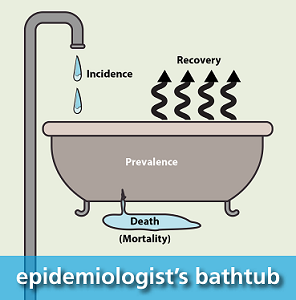
\includegraphics[width=6cm]{static/images/epidemiologists-bathtub.png}
  \end{center}
  \caption{The "epidemiologist's bathtub" \cite{arnold2020}}
  \label{fig:epidemiologists-bathtub}
\end{figure}

Let the bath represent a
set of infected people (those who carry the disease) in certain time.
The size of this set is so-called \textit{prevalence} (sometimes also referred 
as \textit{active cases} number) for that time.
The prevalence can be \textit{increased} or \textit{decreased} when time is shifted upwards.
The increase is referred as the \textit{incidence} (will be mostly denoted $c$ here).
In the case of decrease of prevalence, this may be done in two ways:
the infected individual dies - increase in \textit{mortality}, or, the
infected individual get restored from the disease - get 
\textit{recovered} in terms of epidemiology.
If we do not distinguish the way of decrease, we say the
individual was \textit{removed}.

Basically, from the perspective of specific case, the disease is
transmitted between \textit{infector} $A$ and \textit{infectee} $B$.
The \textit{infector} (also known as \textit{primary case}) is the one who carry the disease and
\textit{infectee} (also known as \textit{secondary case}) is the 
susceptible person, which is being infected.
This abstraction allows to specify several important time intervals.

\begin{figure}[h]
  \begin{center}
    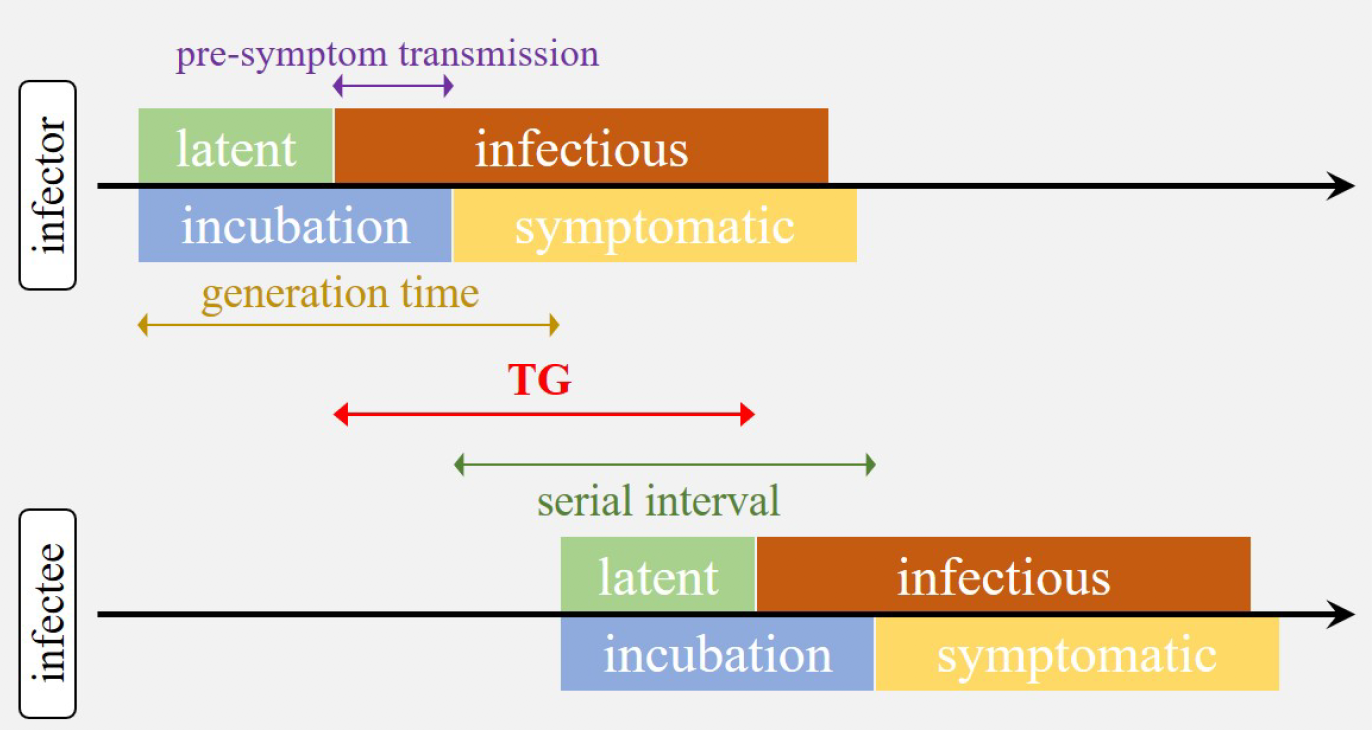
\includegraphics[width=11cm]{static/images/zhao2020_terms.png}
  \end{center}
  \caption{The demonstrative timeline of a transmission chain for a pair of infector and infectee \cite{zhao2020}}
  \label{fig:zhao-transmissive-chain-example}
\end{figure}

These intervals are described in the figure 
\ref{fig:zhao-transmissive-chain-example}.
Most important time intervals are 
\textit{incubation period}, \textit{serial interval} and \textit{generation time}.
\textit{Incubation period} is the time between exposure up to time of onset 
symptoms. Then \textit{symptomatic period} begins.
\textit{Generation time} is the exact time period between 
the infector was infected and the infectee was infected by the infector.
The \textit{serial interval} has similar nature. It is 
the time period between the onset symptoms of the infector 
and onset symptoms noticed on the associated infectee.

% $\phi_h$

% $\phi_s$

% $\phi_g$


% TG, also in the picture \ref{fig:zhao-transmissive-chain-example}, abbreviates 
% \textit{trasmission generation}, which is the time 
% period between the infectiousness of the infector 
% and the infectousness of the infectious, meaning 
% how many susceptibles can be infected from the 
% primary case until the associated secondary case can 
% be transmissibe as well.

TODO: symptomatic vs pre-symptomatic

TODO: \textit{age of infection} is the time for how long the specific individual is infected.

\begin{figure}[h]
  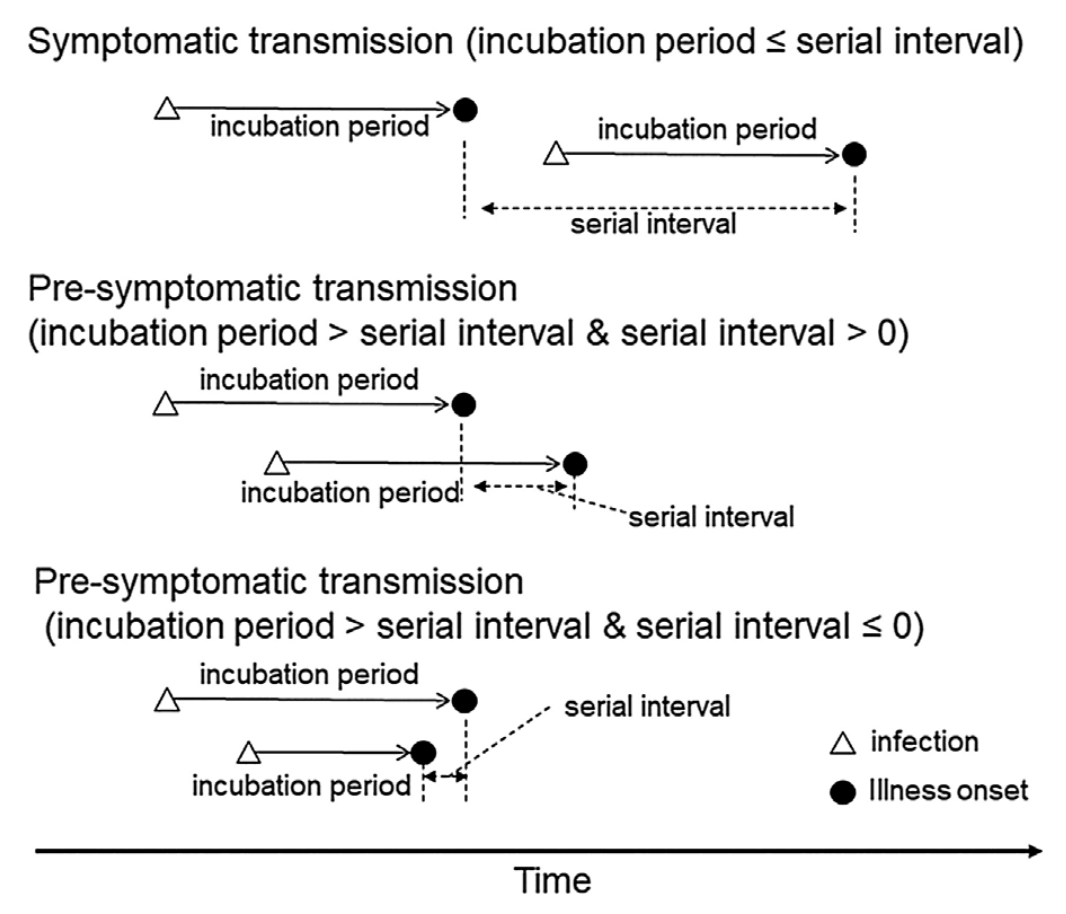
\includegraphics[width=10cm]{static/images/nishiura2020_terms.png}
  \caption{The relationship between the incubation period and serial interval. \cite{nishiura2020}}
  \label{fig:nishiura-transmission}
\end{figure}

In many cases, the serial interval for modeling $\mathcal{R}_t$ 
is used because of its easier determination. 
The main pitfall lies in the possibility of negative serial 
interval, that is when infectee's symptoms are revealed 
earlier than infector's. 
On the other hand, generation time has to be higher than 
zero in its nature, but it is unknown in many cases. 

For example \cite{knight2020} uses deconvolution of incubation 
period and serial interval to obtain generation time.



\section{SIR model}

This is one of the first model, proposed in 1927 by 
William Ogilvy Kermack and Anderson Gray McKendrick, and is 
usually used as an introductionary model to epidemic 
modeling \cite{martcheva2015} due to its simplicity. 
Often serves as a foundation for more complex 
models (\cite{clancy2008} for example).

The SIR model divides entire population into three disjunct 
sets, called \textit{classes} or \textit{compatments} (hence the general 
name \textit{compartment models} \cite{bacaer2011}):

\begin{itemize}
  \item \textit{Susceptibles (size denoted $S$)} - set containing non-infected individuals, but with possibility to become infected.
  \item \textit{Infectious (size denoted $I$)} - individuals who are infected and also able to infect susceptible individuals.
  \item \textit{Removed (size denoted $R$)} - those who was restored from illnes (and gained immunity) or those who died. In both cases, they are removed from susceptibles and infectious sets and the do not play further role.
\end{itemize}

To define the SIR model, let us explain the \textit{force of infection} first.
The force of infection, noted $\lambda$, is similar to 
potential energy in physics, in this case, it expresses 
potential spreading force of the infectious compartment:

\begin{equation}
	\lambda = \tau \rho I
\end{equation}

Where $\rho$ is the average contact rate of person within whole 
population, no matter if they are susceptible, infectious 
or removed. Therefore $\rho N$ is the \textit{average number 
of contacts per unit of time}.
Assuming the susceptibles are independently and identically 
distributed, the probability of selecting any susceptible 
in the population is equal to $\frac{S}{N}$.
Therefore $\rho N\frac{S}{N}$ is the number of contacts 
each infected individual makes with susceptibles 
(simplifies to $\rho S$).
$\tau$ is the probability of becoming infectious for 
susceptible, which met an infected individual:

\begin{equation}
	\tau = p \left( B~\textrm{is infected from}~A~|~B~\textrm{has contact with}~A \right)
\end{equation}

If the previous equations are combined together, 
$\tau \rho S$ can be assumed as the number of 
susceptibles who became infectious after they have 
met one infected individual per unit of time.
Now the incidence may be formulated as:

\begin{equation}
	c = \tau \rho S I = \lambda S
\end{equation}

For practical usages denote $\tau \rho$ as $\beta$ 
and substitute it into previous equation to get:

\begin{equation}
	c = \beta S I
\end{equation}

The compartment models are usually specified as a set of
differential equations. Lets start with the susceptibles
compartment $S$. In the basic SIR model, the $S$
can be decresed only (as it assumes the everyone can be 
infected only once).
This decrease is equal to the incidence, hence:

\begin{equation}
	\frac{\partial{S}}{\partial{t}} = -c = -\beta S I
\end{equation}

The first differential equation for the SIR model has 
been established. It can be interpreted as a decrease 
in size of susceptible compartment which is equal 
to incidence.
The decrease of susceptibles $\beta S I$ is basically 
count of the newly infected individuals, which have 
to be added to $I$. 
Then some of the infected individuals restore from 
the infection or decease. 
This proportion is equal to $\gamma I$, where $\gamma$ 
is called recovery rate. Both increase and decrease in 
the $I$ compartment is caught in equation:

\begin{equation}
	\frac{\partial{I}}{\partial{t}} = \beta S I - \gamma I
\end{equation}

Finally, the decreased proportion $\gamma I$ from the 
$I$ compartment increases removed compartment $R$:

\begin{equation}
	\frac{\partial{R}}{\partial{t}} = \gamma I
\end{equation}

This model has several assumptions:

\begin{enumerate}
  \item Population is constant over time \\
    \begin{equation}
      N = S(t) + I(t) + R(t) = const.
    \end{equation} \\
    Therefore: \\
    \begin{equation}
      \frac{\partial{S}}{\partial{t}} + \frac{\partial{I}}{\partial{t}} + \frac{\partial{R}}{\partial{t}} = 0
    \end{equation}
  \item When susceptible gets infected, it also becomes infectious
  \item Each susceptible has equal probability to become infectious
  \item Everyone can be infected only once in his lifetime
  \item Each infected individual is equally infective \cite{volz2018}
\end{enumerate}



\section{Reproduction number}

The \textit{basic reproduction number} $\mathcal{R}_0$ is number 
of secondary cases caused by the one infectious individual 
in the completely susceptible population and can be expressed
as the following proportion \cite{jones2007}:

\begin{equation}
	\mathcal{R}_0 \propto \left(\frac{infection}{contact}\right)\cdot\left(\frac{contact}{time}\right)\cdot\left(\frac{time}{infection}\right)  
\end{equation}

In terms of SIR model defined above, and the fact $\gamma^{-1}$ is 
the average time of infection, the following formula can be derived:

\begin{equation}
	\mathcal{R}_0 = \tau \rho d = \frac{\beta}{\gamma}
\end{equation}

Note the dimensionlessness of the $\mathcal{R}_0$.

The \textit{effective reproduction number} $\mathcal{R}_e$ 
($\mathcal{R}_{\text{t}}$, $\mathcal{R}_{\text{eff}}$ in 
some literature) is the average number of secondary cases 
caused by the one infected individual within the 
conditions of time $t$ in the ongoing epidemic \cite{chowell2016}:

\begin{equation}
	\mathcal{R}_e(t) = \mathcal{R}_0 \frac{S(t)}{N} = \frac{\beta}{\gamma} \frac{S(t)}{N}
\end{equation}

The basic reproduction number $\mathcal{R}_0$ is usually used
in the early epidemic phase to determine transmission potential.
When infection is
spreading through a population, it is often more convenient
to work with the effective reproduction number $\mathcal{R}_e(t)$.

\section{Exponential growth model}

The severity of epidemic spread can be estimated also by the
\textit{exponential growth rate} $r$. If $r > 0$ the epidemic is growing,
if $r = 0$, then epidemic holds constant incidence, and finally, 
when $r < 0$ the epidemic is weakening in its spread.
In the case of SIR model, the $r$ can be expressed as \cite{ma2019}:

\begin{equation}
  r = \beta - \gamma
\end{equation}

FIXME: From the epidemiological perspective, we can 

\begin{equation}
  I(t) = I_0 e^{rt}
\end{equation}

\section{Wallinga \& Lipsitch model}

Wallinga and Lipsitch \cite{wallinga2007} developed a non-parametric
model (shortened as \textit{WL model} here), which is able to infer
the basic reproduction number from the \textit{exponential growth rate} $r$.

This model is based on the exponential growth model described earlier and
Euler-Lotka equation\footnote{\url{https://en.wikipedia.org/wiki/Euler\%E2\%80\%93Lotka_equation}},
which was originally used to model population dynamics.
Let the $b(t)$ be number of female births in the time $t$, $a$ is 
age of the mother (assuming population has sufficient 
number of males to ensure reproduction, therefore we do not 
count them in), and $n(a)$ is the rate of production of female offsprings 
by one mother at her age $a$. Then we have this equation (which is 
special type of renewal equation \cite{feller1941}):

\begin{equation}
  b(t) = \int_{0}^{\infty} b(t - a) n(a) da
\end{equation}

If we sum up the $n(a)$ in the equation, we obtain \textit{reproductive number} 
$\mathcal{R}$ expressing the total number of female offsprings from one mother:

\begin{equation}\label{eq:wl-model-R}
  \mathcal{R} = \int_0^{\infty} n(a) da
\end{equation}

As the $b(t)$ is assumed to follow exponential growth model, then 
the $b$ functions can be assumed $b(t) = Q e^{rt}$ and 
$b(t - a) = Q e^{r(t - a)} = Q e^{rt} e^{-ra}$, therefore the
previous equation may be rewritten to:

\begin{equation}
  Q e^{rt} = \int_{0}^{\infty} Q e^{rt} e^{-ra} n(a) da
\end{equation}

Note the $Q e^{rt}$ on both sides. At the side of integral and 
as this expression is independent of $a$, i.e., constant, we can 
divide both sides by this constant to obtain Euler-Lotka
equation (in the original equation $n(a) = l(a) m(a)$, but 
here is intentional simplification):

\begin{equation}\label{eq:wl-model-euler-lotka}
  1 = \int_{0}^{\infty} e^{-ra} n(a) da
\end{equation}

To incorporate $\mathcal{R}$ we can normalize the $n(a)$, in the
previous equation, by the equation \eqref{eq:wl-model-R} to get
normalized distribution $\omega(a)$:

\begin{equation}
  \omega(a) = \frac{n(a)}{\int_0^{\infty} n(a) da} = \frac{n(a)}{\mathcal{R}}
\end{equation}

Let the previous be employed in the equation \eqref{eq:wl-model-euler-lotka}:

\begin{equation}\label{eq:wl-model-euler-lotka-R}
  \frac{1}{\mathcal{R}} = \int_{0}^{\infty} e^{-ra} \frac{n(a)}{\mathcal{R}} da = \int_{0}^{\infty} e^{-ra} \omega(a) da
\end{equation}

Finally, we can obtain the formula for computation reproductive number
$\mathcal{R}$ from the exponential growth $r$ and reproduction profile $\omega$:

\begin{equation}\label{eq:wl-model-euler-lotka-R-final}
  \mathcal{R} = \frac{1}{\int_{0}^{\infty} e^{-ra} \omega(a) da}
\end{equation}

In this case $\omega$ fulfills the definition of probability density
(sums up to 1). In the case of epidemiology, $\omega$ represents
distribution of \textit{generation time} defined earlier.
$\mathcal{R}$

\section{Fraser model}

The \cite{fraser2007} proposes model where the effective 
reproduction number $\mathcal{R}_t$ is computed from the 
daily incidence data and generation time only.

The approach of Fraser is very related to WL
model.


The main idea in this model is the number of newly infected 
individuals $c(t)$ in time $t$ is proportional to 
previous prevalent cases $c(t - \tau)$, where 
$\tau > 0$ denotes infection age, and the transmissibility 
$A(t, \tau)$. The infection age describes how long ago 
the particular infection was established in the specific 
individual.
The reason, $A(t, \tau)$ depends on calendar time $t$ is 
the epidemic may change its behavior seasonaly or the 
public restrictions may change during time, for example.
The $\tau$ dependence is given by the age of infection 
since the spreading ability of specific infected individual 
also might be changed during different phases of the 
particular illnes.
Then we can use the convolution over previous cases 
and transmissibility to obtain the expected incidence:

\begin{equation}
c( t ) = \int^{\infty}_0 A ( t, \tau ) c ( t - \tau ) d\tau
\end{equation}

For practical purposes, it is convenient to bound $\tau$ 
by specific $\tau_m$ which may correspond to the maximal 
infection age, assuming nobody is infectious after 
$\tau_m$, therefore $A(t, \tau) = 0$ if $\tau > \tau_m$.
This leads to the next simplification.
For bounded $\tau < \tau_m$, where $\tau_m$ is 
sufficiently small, $A(t, \tau) = A(s, \tau)$ for 
$\forall s \in \left[ t - \tau_m, t \right]$.
Next, Fraser assumes that the seasonal infectivity is 
independent of infection age, therefore the transmissibility 
can be decomposed as:

\begin{equation}
A(t, \tau) = \phi_1(t) \phi_2(\tau)
\end{equation}

The average number of infected cases from the single infected 
individual can be obtained by summing over transmissibility:

\begin{equation}
\mathcal{R}_e = \int^{\infty}_0 A(t, \tau) d\tau = \int^{\infty}_0 \phi_1(t) \phi_2(\tau) d\tau = \phi_1(t) \int^{\infty}_0 \phi_2(\tau) d\tau
\end{equation}

The $\phi_1(t)$ and $\phi_2(\tau)$ might be reweighted as 
product $\phi_1(t) \phi_2(\tau)$, without loss of generality. 
Therefore $\int^{\infty}_0 \phi_2(\tau) d\tau = 1$ may be assumed. 
This bring that $\mathcal{R}_e = \phi_1(t)$, while $\phi_2(\tau)$ 
is considered to be a distribution of infectivity $\tau$ ago, 
meaning idealised generation time distribution $w$. 
Therefore:

\begin{equation}
A(t, \tau) = \mathcal{R}(t) w(\tau)
\end{equation}

Putting it to the renewal equation the following is obtained:

\begin{equation}
  \begin{split}
    c(t) & = \int^{\infty}_0 \mathcal{R}(t) w(\tau) c(t - \tau) d\tau \\
    & = \mathcal{R}(t) \int^{\infty}_0 w(\tau) c(t - \tau) d\tau\\
    & = \mathcal{R}(t) \Lambda(t)    
  \end{split}
\end{equation}

where $\Lambda(t)$ denotes the integral.

For practical usage, we will discretize the previous equation 
and add $\tau_m$ boundary, because of assumption of maximal 
infectious age to be $\tau_m$, and also because of discrete 
observations:

\begin{equation}
c_t = \mathcal{R}_e \Lambda_t = \mathcal{R}_e \sum^{\tau_m}_{\tau=0} w(\tau) c(t - \tau)
\end{equation}

For the sake of simplicity, 

This approach was laterly adopted by \cite{cori2013} where serial 
interval was used as approximation of the generation time.
Also \cite{gostic2020} recommends the approach of \cite{cori2013} 
for the real time $\mathcal{R}_t$ estimation. \cite{knight2020} 
enhances that approach using generation time obtained from 
deconvolution of serial interval and incubation period. 
The method proposed in \cite{hasan2020} uses 
\textit{extended Kalman filter} with comparable results 
to \cite{cori2013}.

This model is mentioned due to its employment in this thesis.

As we want to estimate the number of active cases, both the 
SIR model and Fraser model may be applied. 
Big disadvantage of SIR model is need to estimate its 
parameters which may change over time. 
On the other hand, Fraser model only needs incidence 
data and serial interval to estimate active cases.

TODO: tune up this chapter!

\section{The prevalence estimation}

TODO:



\chapter{The situation analysis}

The purpose of this chapter is to better understand the situation 
we want to model and describe the data as available evidence. 
The modelled infectious disease, Covid-19, is a abbreviated 
term for \textit{coronavirus disease 2019}, the infectious disease 
caused by SARS-CoV-2 virus. 
In december 2019, it was the first time the virus was spotted, 
when several patients with pneumonia was hospitalized in the 
Wuhan, Hubei province in China. 
After the extraction of virus genome, it was discovered 
70\% similarity in genetic sequence with SARS-CoV, 
firstly appeared in China in 2002, the fatality rate 
was 9.6\% \cite{hui2019}.
This was ignition for governments to start with mitigation 
actions.

Covid-19 had huge health and economical impact not only in 
Czechia, but in the whole world. 
Therefore there are various data sources from around the world. 
According to the Fraser model, we need incidence data and 
serial interval.
The incidence data itself corresponds to the geographical 
segment of interest which is often part of official reports, 
but serial interval is usually not.


\section{Serial interval}

To recall, the \textit{serial interval} (SI) $w$ is a time 
interval between onset symptoms on the infector and the 
infectee, and may be expressed as a univariate random variable. 
Although the SI definitely depends on the variant (mutation) of 
Covid-19, the several SI resources from various time periods are 
presented to make a better picture of that distribution.

\cite{simone2020} assumes serial interval to be gamma 
distributed, i.e. $w \sim Gamma(\alpha,\beta)$, where 
$\alpha \sim N \left( 1.87, 0.26^2 \right)$ and 
$\beta \sim N \left( 0.28, 0.04^2 \right)$ in Italia. 
\cite{prete2020} proposes $w \sim LogNormal(\mu, \sigma)$ 
with $\mu = 1.09$ and $\sigma = 0.72$ according to the 
studies in Brazil. The \cite{knight2020} uses deconvolution 
to obtain directly generation interval, which we can use 
as $w$ as well: $w \sim Gamma(\alpha, \beta), \alpha = 1.813, \beta = 2,199$.
\cite{du2020} proposes normally distributed serial 
interval with $\mu = 3.96$ and $\sigma = 4.75$. 
The \cite{nishiura2020} concludes 
$w \sim LogNormal \left( \mu = 4.7, \sigma = 2.9 \right)$.

\begin{figure}[h]
  \begin{center}
    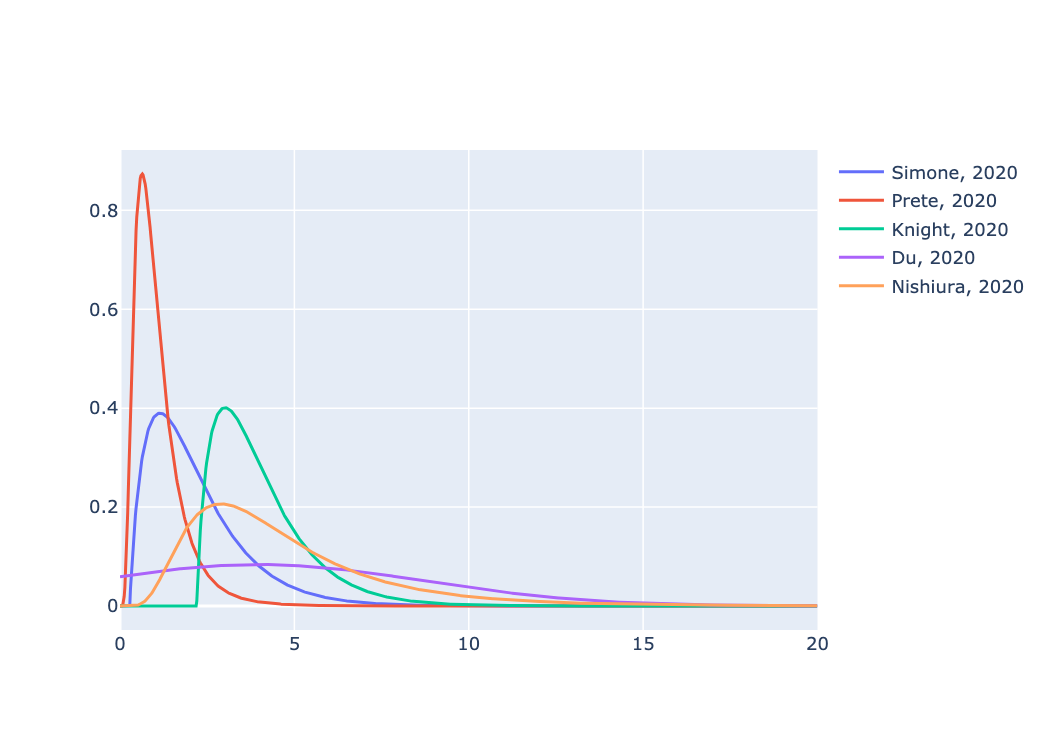
\includegraphics[width=\textwidth]{generated/images/serial-intervals-overview.png}
  \end{center}
  \caption{Referenced serial intervals}
  \label{fig:serial-intervals-overview}
\end{figure}

The previous serial intervals vary due to spatial and 
temporal differences in population composition and the
strain of the virus.
Those are not suitable for Czech republic. 
The \textit{National Institute of Public Health} (NIPH)  
compared Covid-19 to flu\footnote{\url{http://www.szu.cz/tema/prevence/chripka-versus-koronavirus-podobnosti-a-zasadni-rozdily-k-18}}, 
where flu has average SI 3 days, 
Covid-19 5-6 days, moreover, the mortality is 30-40x higher.
From the local research made by \cite{majek2020}, 
it is estimated the SI of Covid-19 for Czech republic is 4-5 days, which is 
consistent with \cite{nishiura2020}. 
In the time of writing this thesis, more precise work on the 
SI of predominant delta mutation could not be found. 
Therefore we will stick with \cite{majek2020} and 
\cite{nishiura2020} and assume 
$w \sim LogNormal \left( \mu = 4.7, \sigma = 2.9 \right)$ 
as the source of truth. 

According the chart above, we can put upper limit of the 
infection age $\tau_m$ to $15$ days.

\section{Available data}

In general, the model is strong as the input data provided.
For epidemic modelling purposes, the most relevant data 
assumed comes from the official authorities.
For the Czech republic, there is a Covid-19 reporting web 
portal\footnote{\url{https://onemocneni-aktualne.mzcr.cz/}} operated 
by the Ministry of Healthcare and developed by IHIS CR\footnote{Institute of Health Information and Statistics of the Czech Republic, \url{https://www.uzis.cz/}} 
and IBA LF MU\footnote{Institute of Biostatistics and Analyses at the Faculty of Medicine of the Masaryk University, \url{http://www.iba.muni.cz/}}, 
stating National Health Information System (NHIS), Regional Public 
Health Authorities (RPHAs) and Ministry of Healthcare as its 
data source. 
The source is updated on the daily basis and provides several 
dataframes with lowest geographical granularity per district.

This data will allow us to compute the risk for each district 
with respect to the chosen serial interval. 
For the modelling the risk, we also need a total population 
$N$ in each investigated district.
In the Czechia, there is 76 districts and the capital city Prague. 
Each district (and Prague) can be uniquely identified by its 
Local administrative unit (LAU) code. 
This will allow us to map it with the official population 
statistics\footnote{\url{https://www.czso.cz/csu/czso/pocet-obyvatel-v-obcich-k-112021}}.

The observed incidence $Y$ for the three largest 
cities in Czechia, namingly Prague, Brno and Ostrava, looks as 
follows:

\begin{figure}[h]
  \begin{center}
    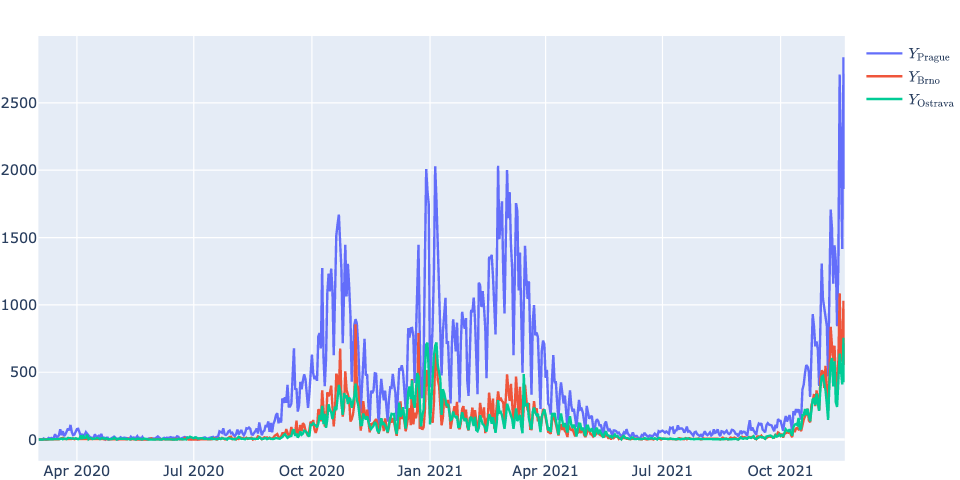
\includegraphics[width=\textwidth]{generated/images/largest-cities-incidence.png}
  \end{center}
  \caption{Observed incidence in the largest cities of Czechia}
  \label{fig:largest-cities-incidence}
\end{figure}


\section{Data analysis}

From the previous plot, it is obvious the data are overloaded 
with noise. 
In the detail view, the weekly seasonal pattern can be observed. 
In the epidemiology, according to \cite{liu2021} and \cite{annunziato2020}, 
those oscillations may be associated to the different capacities 
of testing and reporting delays due to weekends. 
We will assume, this also applies for the Czechia's case of 
Covid-19 reporting, as \cite{komenda2020} and corresponding web 
application authors describe the methods how the data are
collected and processed.


\subsection{Stationarity verification}

As those data correspond to the time series, the stationarity 
should be verified. 
This may be done by Augmented Dickey-Fuller (ADF) test. 
In the  ADF test, the null hypothesis that a unit root is 
present in a sample. 
If the unit root is present, the sample is non-stationary. 
Alternative hypothesis is, therefore, the stationarity of 
the given sample.

\begin{table}
\begin{tabularx}{\textwidth}{lllX}
\toprule
\midrule
ADF Statistic & -1.245 \\
p-value & 0.654 \\
Critical Values &  \\
 & 1\%: -3.441 \\
 & 5\%: -2.866 \\
 & 10\%: -2.569 \\
\bottomrule
\end{tabularx}
\caption{ADF stationary test for Prague incidence data}
\label{tab:adf_test_prague}
\end{table}


In general, p-value is the probability that test statistic 
of unknown distribution has equal or less extreme values 
than unknown distribution of the sample, assuming null 
hypothesis to be true. In simple words, it is the strength 
of belief in the null hypothesis, that the sample is 
non-stationary. 
As that value of p-value is higher than $5\%$, we fail to reject 
the null hypothesis, arguing the observed incidence 
$\Delta C_{\text{Prague}}$ was generated by a non-stationary 
process. 
Of course, the ADF test should be done for $\Delta C_{\text{Brno}}$ 
and $\Delta C_{\text{Ostrava}}$ samples as well, 
see tables \ref{tab:adf-test-brno}, \ref{tab:adf-test-ostrava}.
The results found have the similar nature, i.e.
the time series are non-stationary.

\subsection{Seasonality decomposition}

In the previous subsection, we have found the incidence time 
series data, for the three largest cities, are not stationary. 
This means the specific $\Delta C_i$ was not generated by the 
process with a constant probability distribution over time. 
This brings us to go further and analyze data more precisely. 
For this purposes, the seasonal decomposition may be applied. 
This type of decomposition results in structural time series, 
where the input time series is decomposed into specific 
components.

In this case, the decomposition is done by computing 7 days 
two-sided moving average as a trend component $T$, then the 
seasonal component $S$ and residual $\epsilon$ is inferred. 
How the components are inferred depends on the selected model 
of decomposition. There are two considerable types: 
\textit{additive} and \textit{multiplicative}.

The following figures shows decomposed daily incidence 
$\Delta C$ to structured time series components. 
First figure show the additive decomposition model, 
formally $\Delta C = T + S + \epsilon$:

\begin{figure}[h]
  \begin{center}
    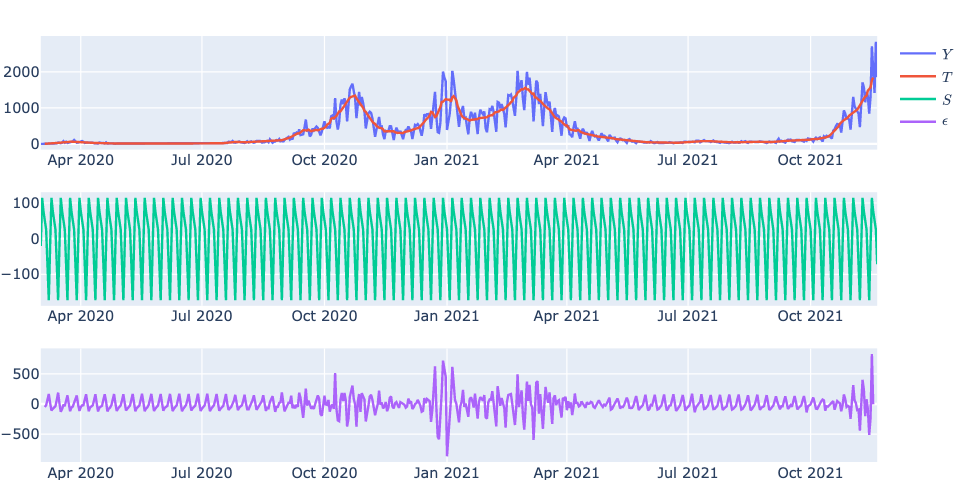
\includegraphics[width=\textwidth]{generated/images/seasonal-decomposition-additive.png}
  \end{center}
  \caption{Example of additive seasonal decomposition}
  \label{fig:seasonal-decomposition-additive}
\end{figure}

Similarly, the second figure shows the multiplicative 
decomposition, particularly $\Delta C = T S \epsilon$:

\begin{figure}[h]
  \begin{center}
    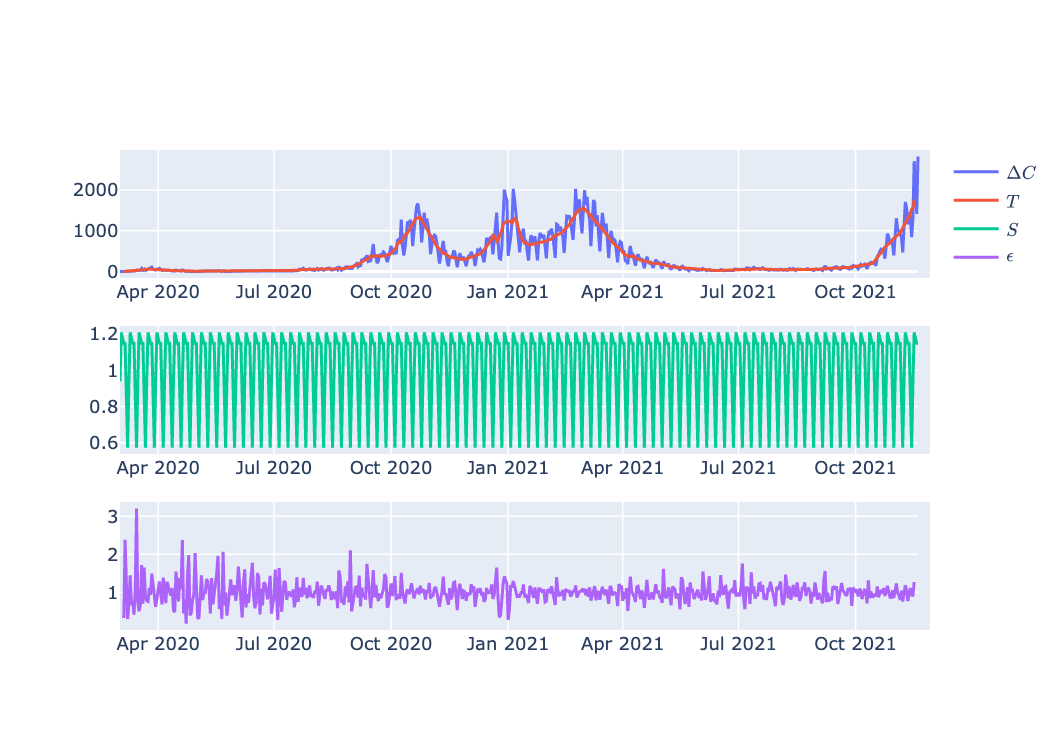
\includegraphics[width=\textwidth]{generated/images/seasonal-decomposition-multiplicative.png}
  \end{center}
  \caption{Example of multiplicative seasonal decomposition}
  \label{fig:seasonal-decomposition-multiplicative}
\end{figure}

From the previous plots, we can see rather the multiplicative 
relationship, according to residual component $\epsilon$, 
which distinctly acts more stationary right in the 
multiplicative model. 
The multiplicative model imply the variance is dependent 
on the mean. This effect can be, after all, also seen 
in the raw source data.

To conclude, the data analysis shown multiplicative 
relationship between trend, seasonality and residual 
components in the incidence data. 
The input data are very noisy and non-stationary, which 
usually eliminates many well-known deterministic, therefore 
fast, statistical methods. 
They usually suffer from poor input data, so the data have 
to be somehow preprocessed first, otherwise the poor 
approximations are produced out of these methods.

The noisiness in the data can be overcome by using 
smoothing techniques.
\cite{elmousalami2020} compares moving average, weighted 
moving average, single exponential smoothing for 
forecasting Covid-19, while these methods may be used 
for smoothing too. 
Downside is loss of information about uncertainty by using 
those methods. 
Also \cite{annunziato2020} draws attention to use smoothing 
methods carefuly as some oscillations may still remain in 
the input data, thus the risk may be estimated imprecisely.

To overcome previous issues, the thesis offers the robust 
probabilistic solution.



\chapter{The incidence model}

In the most basic taxonomy of mathematical models, they can be 
split into two main categories: \textit{deterministic} and 
\textit{probabilistic}, also known as \textit{stochastic}. 
Big advantage of deterministic models is their 
straightforwardness and lower computational demands. 
On the other hand, they bring one huge pitfall - very 
poor options to display uncertainty and usually higher 
sensitivity to the input data. 
The deterministic approach usually results in a numerical 
value, often with some deviation, but it miss the idea 
how certain we are about the oscillation of a random 
variable around its mean. 
In the probabilistic approach, the value is represented 
by its probability distribution, so the idea about 
certainty in the value of variable is available. 
The probabilistic modelling is based on the Bayesian 
way of thiking.

\section{The Bayesian approach}

The Bayesian way of thinking is more similar to how human 
brain works in contrary to the frequentistic approach. 
Usually, we, as humans, have some prior belief about some 
unknown quantity or event, and whenever we obtain new 
evidence, we update our belief forming the posterior, such 
that the next time we obtain new evidence, this posterior 
is used as a new prior, etc. 
Technically, everytime someone asks us about or opinion 
about the quantity, we are expressing our latest posterior 
about that quantity. 
Therefore, more evidence we have collected about the 
quantity during our life, the stronger our belief in 
that quantity is.

Let's image a toy example with coin tossing. 
Initially, before we toss the coin, we have no reason 
to think the coin is not fair, so we put our prior belief 
in tossing a head to $50\%$ and obviously tail to 
$50\%$ as well. 
But, if we start tossing and we obtain 8 tails in a row, 
we may start to believe the coin is biased. 
In reality, we should toss the coin very many (ideally 
infinitelly many) times to confirm its fairness, but 
by doing this, we fall back to frequentistic way of 
thinking. 
The Bayesian approach basically allows to be 
"more subjective" regarding to evidence we obtained. 
Therefore it practically better fits situations with 
less data available.

Formally, let $X$ be a random variable representing 
the unknown quantity and $Y$ the random variable for 
the observed quantity, therefore we can express $p(X)$ 
as a prior distribution of the unknown quantity and 
$p(Y)$ as a probability distribution of evidence. 
Posterior distribution can be expressed in terms of 
conditional probability such that $p(X | Y)$, meaning 
what is the probability distribution of $X$ given we 
know/observe $Y$. 
This posterior can be obtained using the Bayes 
theorem:

FIXME: place nice pic here instead of this

\begin{equation}
p( X | Y ) = \frac{p( Y | X ) p(X)}{p(Y)}
\end{equation}

where the $p( Y | X )$ is called the *likelihood*. 
Note the likelihood is reverse to posterior, i.e. it 
is a probability distribution of evidence given the 
knowledge of $X$. 
In practice, it is hard to think about/ express the 
probability distribution of evidence $p(Y)$, it would 
mean we can somehow obtain all possible evidence, which 
is usually not available. 
Instead of this, the $p(Y)$ can be obtained by 
marginalization over the $X$, referred as a 
\textit{normalizing constant}:

\begin{equation}
p(Y) = \int p( Y | X ) p(X) dX
\end{equation}

Unfortunatelly, the integral is usually not easily 
analytically tractable. 
This makes the Bayesian approach quite complex, 
however, during last decades, there was a huge leap 
in development of methods capable of solving this 
(both deterministically and stochastically). 
Choosing the proper solving method depends on the 
defined model, so let's start with the model first.


\section{The probabilistic model}

\subsection{Likelihood}

As the daily incidence is discrete count variable, 
therefore the discrete probabilistic distributions are 
considerable as a likelihood. One of the first suggestions 
might be the \textit{Poisson} distribution. Unfortunatelly, random 
variable $X$ following the Poisson distribution with 
parameter $\lambda$ has very strong assumption 
$\lambda = \mathbb{E}\left[ X \right] = \mathbb{V}\left[ X \right]$, 
which may not be always hold for the input data. 

This is also the our case. 
For this reason, the \textit{negative binomial distribution} can 
be used as the two-parameter substitute for 
one-parameter Poisson distribution to better 
handle overdispersion in the data, similarly 
as \cite{simone2020}, \cite{wallinga2004}, 
\cite{alzahrani2018} and \cite{manevski2020} did.
The following will be our desirable likelihood:

\begin{equation}
c \sim NegBin\left( \mu, \alpha \right)
\end{equation}

Usually, the negative binomial distribution is 
written in the form $NegBin \left( r, p \right)$, 
where $r$ is the number of successful Bernoulli 
trials and $p$ is probability of success in one 
trial. The negative binomial distribution above 
is in the form of conjugate distributions, namely 
$Poisson\left( \lambda \right)$ as a likelihood 
and $\lambda \sim Gamma\left( \alpha, \beta \right)$ as 
conjugate prior \cite{munezero2020}. 
Then, the probability mass function of such 
negative binomial distribution is following:

\begin{equation}
f \left( x; \mu, \alpha \right) = \frac{\Gamma \left( \alpha + x \right) }{x! \Gamma \left( \alpha \right)} \left( \frac{\alpha}{\mu + \alpha} \right)^{\alpha} \left( \frac{\mu}{\mu + \alpha} \right)^{x}
\end{equation}

where $\mu = \frac{pr}{1-p}, \mu \geq 0$ and 
$\Gamma$ is the \textit{gamma function}. 
First parameter of the prior Gamma distribution 
$\alpha = r$ is assumed exponentially distributed:

\begin{equation}
	\alpha \sim Exponential \left( \lambda_{\alpha} \right)
\end{equation}

TODO: fix notation

\begin{equation}
p(\hat{c}|y) \propto p(y|\alpha, \theta, a, b) p(\alpha) p(\theta) p(a) p(b)
\end{equation}

As the previous analysis shown significant 
correlation between mean and variance, the 
logarithmic transformation may be applied, 
formally $log\left( \mu \right) = \theta$. 
The following plot show the original data 
before and after the logarithmic transformation:

\begin{figure}[h]
  \begin{center}
    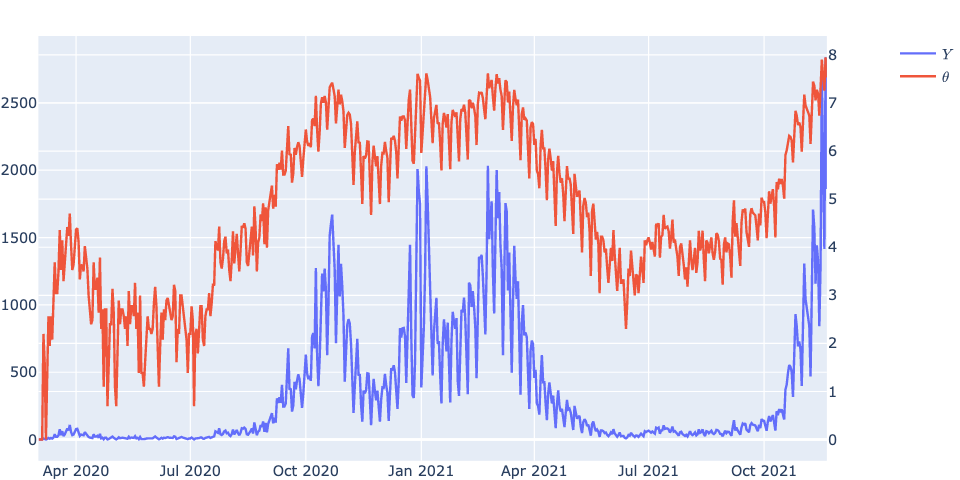
\includegraphics[width=\textwidth]{generated/images/incidence-log-transform.png}
  \end{center}
  \caption{Log transformation of daily incidence}
  \label{fig:incidence-log-transform}
\end{figure}


\subsection{The analysis of \texorpdfstring{$\theta$}{Lg}}

After the transformation, $\theta$ is no 
longer discrete random variable, rather 
continous, but, as the figure shown, it 
is more homoscedastic, which is more 
convenient, because the more homoscedatic 
the random variable is, the more constant variance 
it has. 
This can be verified by detrending/decumulation 
of the $\theta$, to obtain differences 
$\Delta \theta$ with succesive application of 
$\Delta \theta_t = \theta_{t+1} - \theta_{t}$:

\begin{figure}[h]
  \begin{center}
    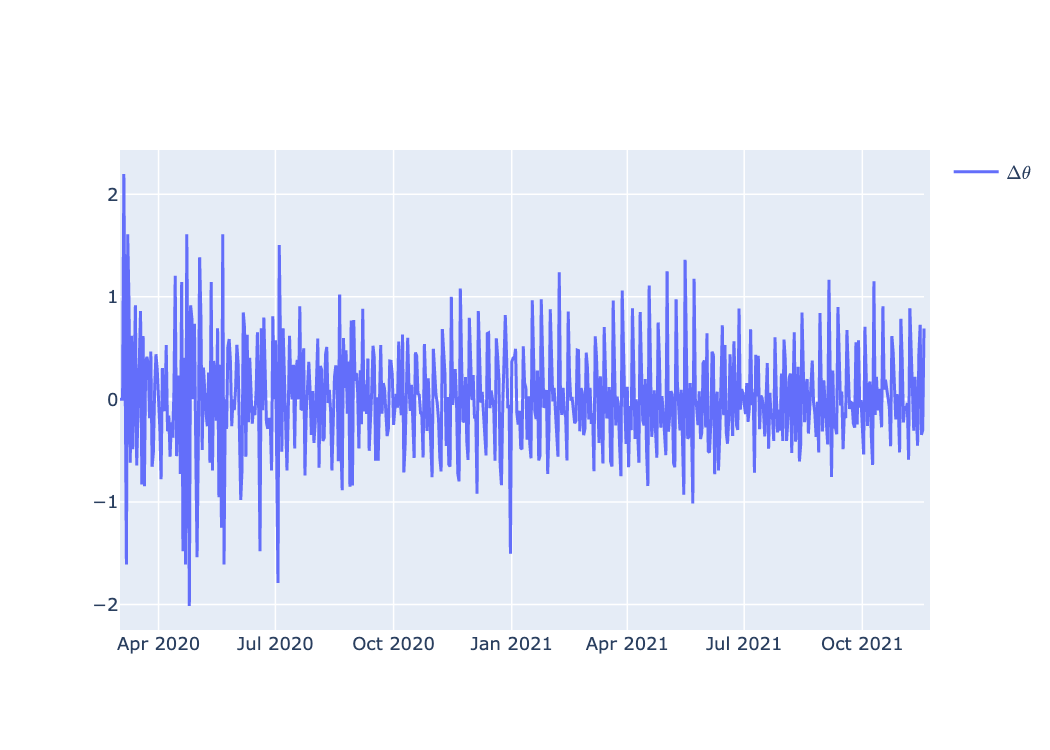
\includegraphics[width=\textwidth]{generated/images/theta-diff-figure.png}
  \end{center}
  \caption{The plot of $\Delta \theta$}
  \label{fig:theta-diff}
\end{figure}

Naturally, we could check normality of the 
whole data, but practically, we work just in 
specific time windows, therefore it will be 
more meaningful to verify normality for those 
windows. In our case, we picked three samples 
of time window as the following figure presents:

\begin{figure}[h]
  \begin{center}
    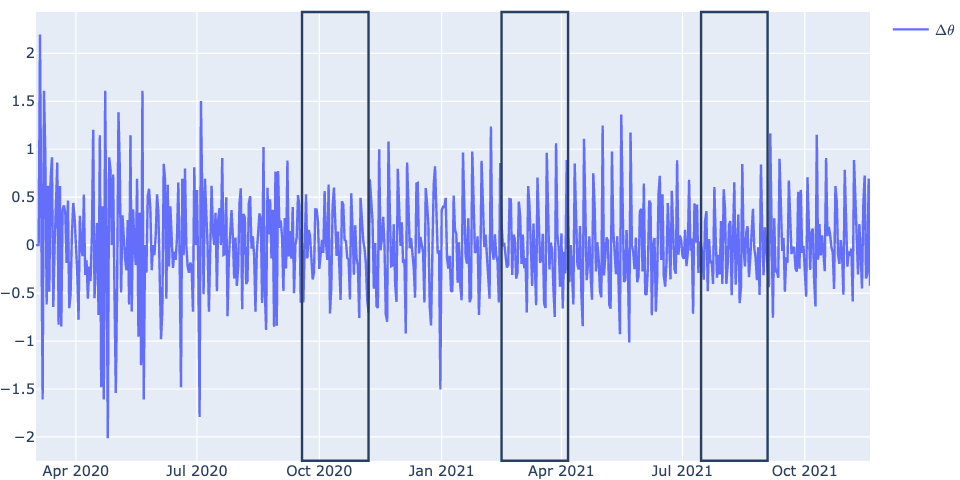
\includegraphics[width=\textwidth]{generated/images/theta-sample-windows.png}
  \end{center}
  \caption{The referenced windows for taking samples of $\Delta \theta$}
  \label{fig:theta-sample-windows}
\end{figure}

Let's explore the distribution of those samples 
for confirmation of normality. 
For visual testing of normality, histogram, 
Q-Q and ECDF/CDF plots may be considered. 
Let's start with histograms:

\begin{figure}[h]
  \begin{center}
    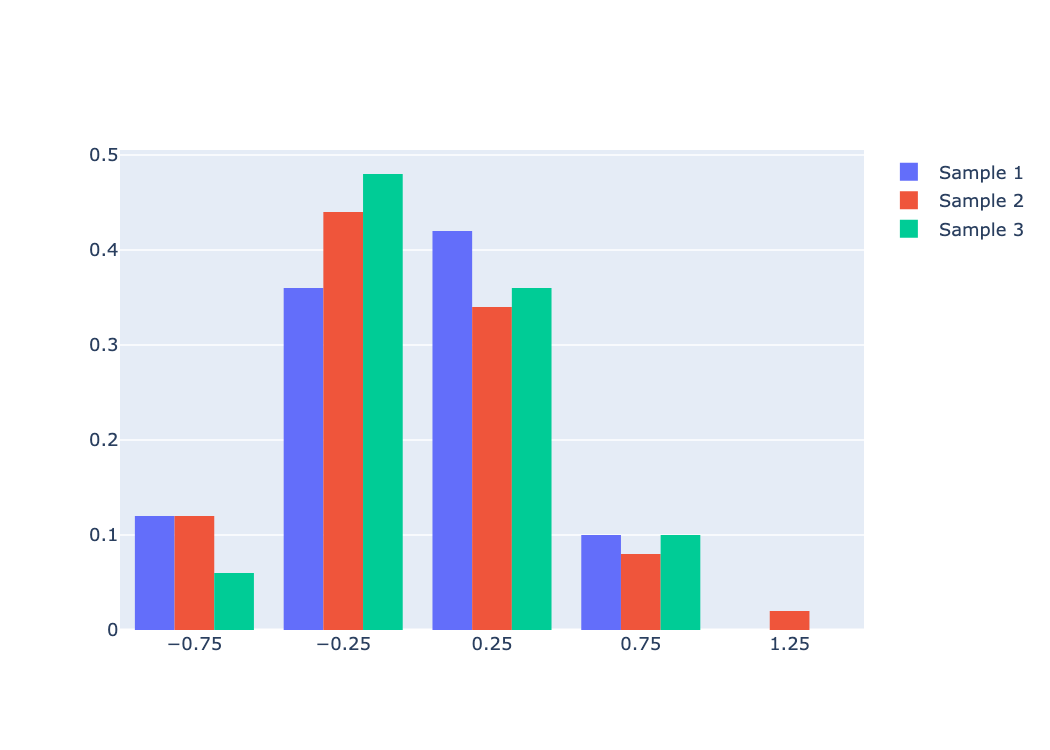
\includegraphics[width=\textwidth]{generated/images/theta-diff-histogram.png}
  \end{center}
  \caption{The histogram of chosen $\Delta \theta$ samples}
  \label{fig:theta-diff-histogram}
\end{figure}

\begin{figure}[h]
  \begin{center}
    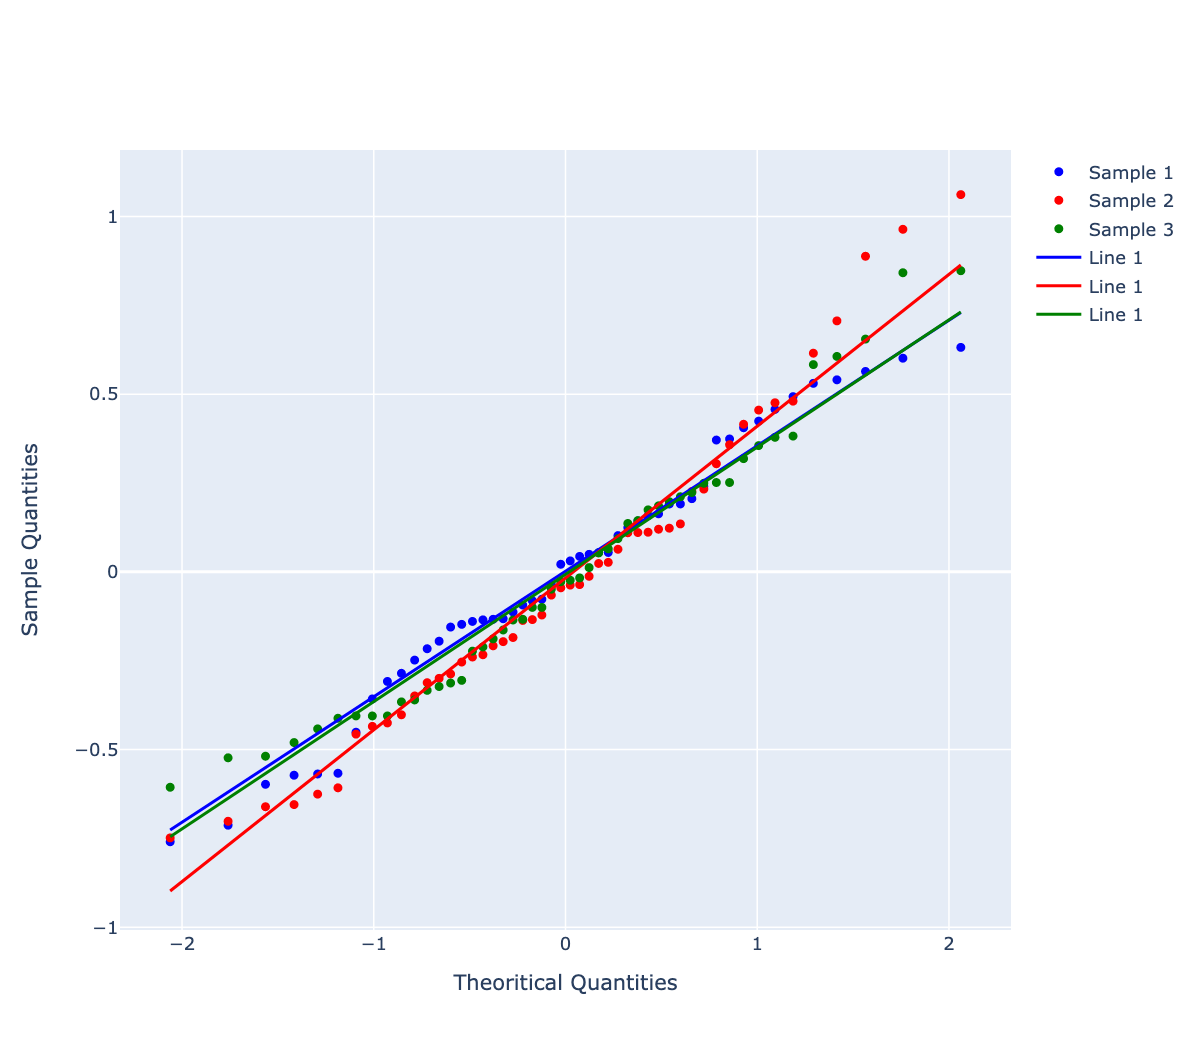
\includegraphics[width=\textwidth]{generated/images/theta-diff-qq.png}
  \end{center}
  \caption{Quantile-Quantile plot of $\Delta \theta$ samples}
  \label{fig:theta-diff-qq}
\end{figure}

\begin{figure}[h]
  \begin{center}
    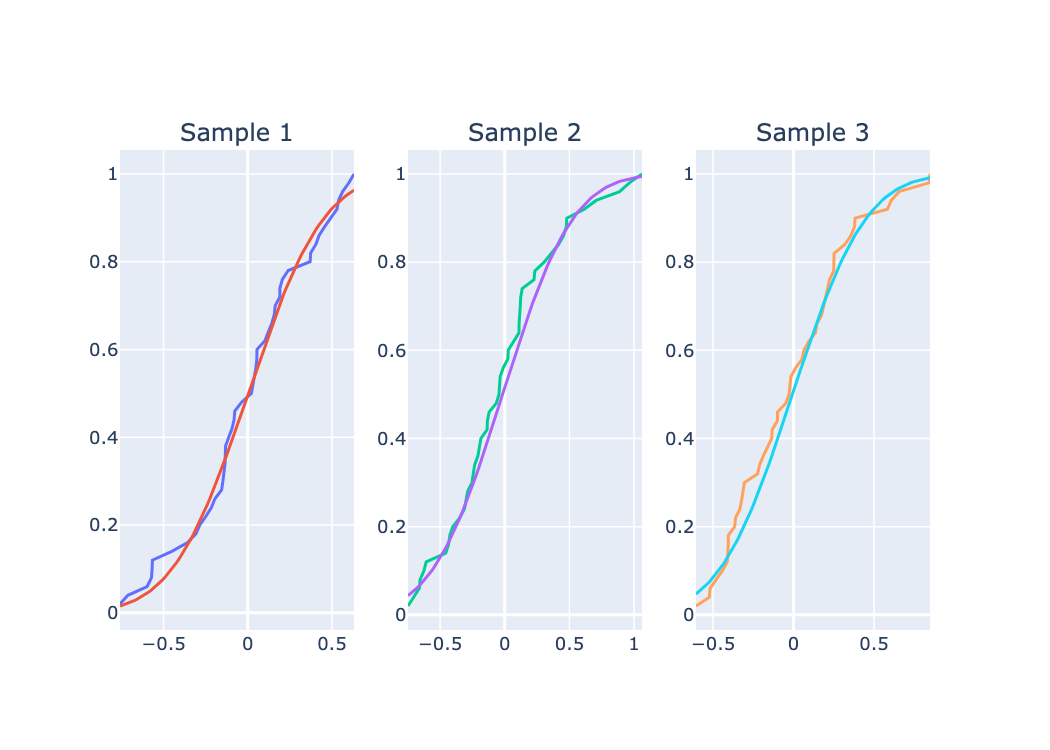
\includegraphics[width=\textwidth]{generated/images/theta-diff-ecdf.png}
  \end{center}
  \caption{Empirical CDF of $\Delta \theta$ samples}
  \label{fig:theta-diff-ecdf}
\end{figure}

From the histogram, the normality is not 
very obvious. 
The main pitfall of histogram is the problem 
of choosing the proper bin size, which we may 
think of as some kind of parameter. 
To narrow bin size means a lot of bins, which 
require a lot of data. 
Too wide bins, on the other hand, ends with 
few bins in the visualisation and we might 
oversee gaps in the data. 
The Q-Q plot is better in this way, because 
it can be assumed as a non-parametric 
visualisation, moreover, we see how all data 
points fit to the normal distribution:

This may finally remind the normally distributed 
data, because closer the points are to the line, 
the more normal distribution is approached in 
the data.

The next plot visualizes the 
\textit{empirical cumulative distribution function}
(ECDF) based on $\theta$ and CDF for the 
theoretical normal distribution based on 
the summary statistics of $\theta$.

The previous visuals might evoke normally 
distributed data for some individuals, but 
visual check might be misleading, therefore 
it should not be sufficient for statistical 
modelling. Instead of visual check, the 
tatistics provides several non-parametric 
normality tests. For the purpose of normality 
testing, Kolmogorov-Smirnov, Lilliefors and 
Shapiro-Wilk tests were performed.

\input{generated/tables/theta-diff-ks-test}
\input{generated/tables/theta-diff-lilliefors-test}
\input{generated/tables/theta-diff-shapiro-wilk-test}

The strongest result is noted in the 
Lilliefors test, then Shapiro-Wilk test and 
worst result is from Kolmogorov-Smirnov test, 
which, lead even to accepting alternative 
hypothesis about non-normally distributed data. 
The research of \cite{razali2011} concludes the 
Shapiro-Wilk test to be the most powerful 
normality test and the Kolmogorov-Smirnov test 
to the least powerful (Kolmogorov-Smirnov, 
Shapiro-Wilk, Anderson-Darling and Lilliefors 
tests were compared). 
According to this research and the fact we 
use limiting infection age $\tau_m$, the 
assumption about normally distributed $\theta$ 
can be made.

To recall, the normality assumption was made 
on the differences $\Delta \theta$, when trend 
was removed by decumulation, but what we need 
is to model prior distribution for the original 
$\theta$, where trend is present. 
This means, for each $\theta_t$ in specific 
time window, the normal distribution may differ 
in its parameters across the time 
$\theta_t \sim N(\mu_t, \sigma_t)$. 
Therefore we can model prior for $\theta$ as a 
\textit{Gaussain process}:

\begin{equation}
\theta \sim GP \left( m \left( x \right), k \left( x, x' \right) \right)
\end{equation}



\subsection{The \texorpdfstring{$\theta$}{Lg} as a Gaussian process}

Generally speaking, Gaussian process 
\cite{rasmussen2004} is a finite set of random 
variables 
$X = (x_1, x_2, \dots, x_n) \in \mathcal{X}^n$ 
corresponding to the multivariate normal 
distribution defined as:

\begin{equation}
X \sim MN \left( m \left( x \right), k \left( x, x' \right) \right)
\end{equation}

where $m$ is the \textit{mean function} and $k$ is the 
\textit{kernel function}. 
The mean function 
$m : \mathcal{X} \to \mathcal{R}$ captures the 
trend in the data for the point $x$ and the 
kernel function 
$k : \mathcal{X} \times \mathcal{X} \to \mathcal{R}^{+}$ 
is actually \textit{Mercer kernel}, also called 
\textit{positive-definite kernel} \cite{murphy2021}, 
measuring how two inputs $x$ and $x'$ are similar. 
This requires the kernel to be symmetric, i.e. 
$k \left( x, x' \right) = k \left( x', x \right)$.

For the sake of simplicity, we will assume linear 
trend between datapoints, therefore function 
$m$ will be like:

\begin{equation}
m(x) = b + a x
\end{equation}

where the prior distributions for $a$ and $b$ 
are assumed 
$a \sim N \left( \mu_a, \sigma_a \right)$ and 
$b \sim N \left( \mu_b, \sigma_b \right)$.

The most widely used kernel is \textit{Gaussian kernel}, 
also called \textit{squared exponential kernel} or 
\textit{radial basis function (RBF) kernel} defined as:

\begin{equation}
k_{RBF} \left( x, x'; \ell \right) = exp \left[ -\frac{(x - x')^2}{2\ell^2} \right]
\end{equation}

where $\ell$ is the \textit{length scale} hyperparameter, 
known also as \textit{bandwidth}. 
This hyperparameter is distance which we expect 
differences to matter.

TODO: $\eta$
TODO: properties of this kernel and reason why it is used here


\section{Monte Carlo simulation}

Simulation itself is relatively old technique for 
solving analytically intractable problems. 
The first such a problem considered is the 
\textit{Buffon's needle problem}\footnote{\url{https://en.wikipedia.org/wiki/Buffon\%27s_needle_problem}} from 1733. 
The probem is defined as probability of the 
needle of length $l$ dropped onto the floor 
represented by parallel strips of distance 
$d$ crosses the line between two adjacent 
strips. 
The analytical solution was discovered in 1777, 
however, the simulation can be done just via 
dropping the needles on the floor and count 
the intersections to calculate probability 
in a frequentistic way.

A huge development in simulation techniques 
came with the development of computers, 
especially during the Los Alamos research 
\cite{metropolis1987}, where 
\textit{Monte Carlo simulation} was invented to 
solve nuclear fission problem - Stan Ulam 
came up with an idea of Monte Carlo simulation, 
John von Neumann with the machine and 
Nicolas Metropolis with the algorithm described 
further.
In fact, the name Monte Carlo refers to the city 
in Monaco, which is famous for its casinos. 
In the casinos, generally, the probability and 
randomness together plays big role, just like in the 
Monte Carlo simulation.

Monte Carlo methods can be used for various 
purposes. 
Most common usage is to estimate the value of 
unknown quantity in terms of inferential 
statistics, meaning the quantity which is not 
directly observable from data.

FIXME: rewrite this part

Most common is the \textit{Monte Carlo integration}, 
i.e. solving analytically intractable integral 
by Monte Carlo techniques. 
Let's imagine we have a random variable 
$x \in \mathcal{X}$ distributed according to 
$\pi$ and we are interested in its expected 
value $\mathbb{E}_{\pi}$. 
The usuall approach would be:

\begin{equation}
\mathbb{E}_{\pi}\left[ f(x) \right] = \int_{\mathcal{X}} \pi \left( x \right) f \left( x \right) dx
\end{equation}

But in many cases, the $\pi$ is not directly 
observable (we do not have all the possible data). 
The Monte Carlo may approach this value by 
generating $n$ independent identically distributed 
random samples $x_i$ (if sampling from $f$ is 
possible) from domain $\mathcal{X}$ to form a 
sample mean of that unknown quantity:

\begin{equation}
\hat{\mu}_n = \frac{1}{n} \sum_{i=1}^{n} f \left( x_i \right)
\end{equation}

According to the unknown quantity above, this 
is its \textit{unbiased Monte Carlo estimator}, i.e. 
estimator of the expected value. 
As $n \to \infty$, from the law of large numbers, 
we can state 
$\hat{\mu}_{\infty} = \mathbb{E}_{\pi}\left[ f(x) \right]$, 
therefore for very large $n$ it holds 
$\hat{\mu}_n \approx \mathbb{E}_{\pi}\left[ f(x) \right]$.

In this approach, the samples are trully 
random meaning independent of each other, 
therefore it is often called 
\textit{random sampling}. 
The main pitfall in random sampling is its 
inefficiency, i.e. slow convergence in terms 
of computational efficiency, moreover, we 
need $n$ to be a very large number to be 
sure the samples sufficiently cover 
$\mathcal{X}$, even for high unprobable values. 
Fortunatelly, by years, several algorithms 
solving this issue were invented. 
In particular, most referred methods are 
so-called \textit{Markov chain Monte Carlo} (MCMC) 
methods.


\subsection{Markov Chain Monte Carlo}

Markov Chain Monte Carlo (MCMC) is a class of 
algorithms solving problem with sampling from a 
\textit{target probability distribution} in more 
efficient way. 
Basic principle is to random walk through 
distribution similarly as random sampling 
does, moreover, samples follow the values 
from areas with higher probabilities which is 
done using the Markov Chain as some kind 
of short-term memory. 
The probability of samples generated by 
MCMC methods are proprotional to the the 
probabilities of the target distribution in 
the long run of particular Markov chain, 
therefore, we can rewrite Bayes theorem to:

\begin{equation}
p( X | Y ) \propto p( Y | X ) p(X) \Rightarrow p( X | Y ) = \alpha p( Y | X ) p(X)
\end{equation}

where $\alpha$ can be computed from the chain. 
MCMC methods differ in the way how they favour 
higher probability areas, however, in their 
underlaying structures, they usually somehow 
follow the basic Metropolis algorithm (also 
often with Hasting's modification).

TODO: incorporate interesting \cite{beichl2000} article

\subsection{Metropolis algorithm}

The algorithm is named after his inventor, 
Nicolas Metropolis, and is very first Monte 
Carlo algorithm utilizing Markov chains 
\cite{metropolis1953}, therefore, first 
MCMC algorithm considered.
Lets imagine, we are interested in theoretical 
probability distribution $\pi(\theta)$ of 
some parameter $\theta$. 
The idea is to gradually generate the 
$\theta^\prime$ parameter into the sequence 
forming Markov chain. 
The generation is done with proposal distribution 
$g(\theta^\prime | \theta_{i-1})$, which is 
conditionally dependent on the last sample 
$\theta_{i-1}$ in the forming Markov chain 
(thus first-order Markov chain), to form 
next sample in this chain. 
The whole process is summarized in the 
following steps. As the initial state 
$\theta_0$, we usually put our initial prior, 
which affects the speed of convergence - 
more accurate the prior is, the faster the 
convergence.

In the step 2, the parameter proposal $\theta^\prime$ 
is being generated, where, in the step 3, is used 
to compute acceptance probability $\alpha$:

\begin{equation}\label{eq:metropolis-alpha}
  \alpha = min\left(1, \frac{f(\theta^\prime)}{f(\theta_{i-1})}\right)
\end{equation}

This probability is then compared with uniformly generated number in
the interval $(0, 1]$ to decide whether accept the 
sample or not. This may look a little bit cumbersome, 
when we may accept parameter $\theta^\prime$ with 
lower probability than $\theta_{i-1}$, but the 
whole idea of acceptance probability is to let 
explore further areas of state space to prevent 
stuck in local minimum, however, the areas with 
higher probability are still prefered.


Input: initial state $\theta_0$

\begin{enumerate}
  \item Set $i \leftarrow 1$
  \item Generate proposal $\theta^\prime \sim g(\cdot | \theta_{i-1})$
  \item Compute acceptance probability $\alpha$ according to \eqref{eq:metropolis-alpha}
  \item Generate $u \sim \text{Uniform}(0, 1)$
  \item Set $\theta_{i} \leftarrow \begin{cases}
    \theta^\prime, & \text{ if } u \leq \alpha,\\
    \theta_{i-1}, & \text{ ow.}
    \end{cases}
    $
  \item Set $i \leftarrow i + 1$ and go to step 2
\end{enumerate}


After the sufficient amount of steps, the Markov 
chain should approximate the stationary target 
distribution $\pi(\theta)$. These number of 
sufficient steps defines \textit{burnin period}, 
referencing the samples being discarded. This 
is happening because it usually takes a while 
until the parameters converge to form 
stationary distribution - it largely 
depends on the choice of prior as was mentioned. 
Basically we take last $n$ samples of the 
stationary distribution depicted by the 
Markov chain.


\subsection{Metropolis-Hastings algorithm}

Is basically enhancement of the Metropolis algorithm 
for asymetric proposal distributions introduced by 
Wilfred K. Hastings in 1970. 
The only modification is the computation of the acceptance 
probability $\alpha$, newly computed as:

\begin{equation}
  \alpha = min\left(1, \frac{f(\theta^{\prime})}{f(\theta_{i-1})} \frac{g(\theta_{i-1} | \theta^{\prime})}{g(\theta^{\prime} | \theta_{i-1})}\right)  
\end{equation}

Notice the change in adding multiplication by fraction 
$\frac{g(\theta_{i-1} | \theta^{\prime})}{g(\theta^{\prime} | \theta_{i-1})}$ 
which is the underlying extension above basic Metropolis 
algorithm...TODO


\subsection{Hamiltonian Monte Carlo}

Hamiltonian Monte Carlo (HMC) is another Metropolis-Hastings 
based algorithm, moreover, it utilizes physical analogy to 
help converge faster \cite{betancourt2018}. 
It started with Hybrid Monte Carlo paper \cite{duane1987}, 
which utilized Monte Carlo to understand the structure 
of atoms. 
The Radford Neal laterly recognized the potential of 
this method during his focus on Bayesian neural networks 
within his doctoral thesis \cite{neal1995}. 
After a few years, it was referenced by some literature, 
until the review of Neal again \cite{neal2011} and availability 
of high performance software to such a computation.

In Hamiltonian dynamics, state is characterized by the
\textit{position vector} $q$ and the \textit{momentum vector} $q$,
both are $d$-dimensional, hence $2d$-dimensional state.
We usually describe this system by the function of
this state $H(q, p)$, called \textit{Hamiltonian}.

Hamilton’s equations describe how $q$ and
$p$ change in time $t$ by the partial derivatives \cite{neal2011}:

\begin{equation}
  \frac{\partial q_i}{\partial t} = \frac{\partial H}{\partial p_i}
\end{equation}

\begin{equation}
  \frac{\partial p_i}{\partial t} = - \frac{\partial H}{\partial q_i}
\end{equation}

The Hamiltonian $H$ can be tought as a total energy in the system,
i.e. sum of \textit{kinetic energy} $K$ and \textit{potential energy} $U$:

\begin{equation}
  H(q, p) = U(q) + K(p)
\end{equation}

The $U$ is assumed as log probability density of the distribution
of position vector $q$ we want to sample from.

Kinetic energy $K$ is assumed as to be $p^\intercal M^{-1} p$, 
where $M$ is mass matrix, which is diagonal, i.e. with
diagonal elements $2m_1, ..., 2m_d$, therefore the computation of $K$
can be simplified:

\begin{equation}
  K(p) = \sum_{i=1}^{d} \frac{p_i^2}{2 m_i}
\end{equation}

TODO: Euler integration

The leapfrog integration:

\begin{equation}
  p_i \left(t + \frac{\epsilon}{2} \right) = p_i(t) - \frac{\epsilon}{2} \frac{\partial U}{\partial q_i} (q(t))
\end{equation}

\begin{equation}
  q_i(t + \epsilon) = q_i(t) + \epsilon \frac{p_i \left(t + \frac{\epsilon}{2} \right)}{m_i}
\end{equation}

\begin{equation}
  p_i(t + \epsilon) = p_i \left( t + \frac{\epsilon}{2} \right) - \frac{\epsilon}{2} \frac{\partial U}{\partial q_i} \left( q \left( t + \epsilon \right) \right)
\end{equation}

From the perspective of statistical mechanics, the $H$ can be seen
as a joint probability distribution

\begin{equation}
  P(x) = \frac{1}{Z} exp \left( \frac{-E(x)}{T} \right)
\end{equation}

\begin{equation}
  P(q, p) = \frac{1}{Z} exp \left( \frac{-H(q, p)}{T} \right)
\end{equation}

\begin{equation}
  P(q, p) = \frac{1}{Z} exp \left( \frac{-U(q)}{T} \right) exp \left( \frac{-K(p)}{T} \right)
\end{equation}

\subsection{No U-Turn Sampler}

\section{PyMC}

PyMC3 is probabilistic programming tool, more specifically, 
it is a Python package capable of Bayesian statistical 
inference using both stochastic and deterministic algorithms. 
The PyMC3 is built upon a Theano (currently fork of 
Theano called Aesara, because Theano is not developed anymore), 
which basically allows to describe mathematical operations in 
high level fashion. 
Those are then transformed to the low level instructions to 
support efficient processing by CPU(s) or GPU(s), just then 
those operations are being executed. 
This is kind of similar to query planning and execution in 
relational databases.

PyMC3 offers MCMC and variational inference methods.
The MCMC includes Metropolis–Hastings (which is its default 
engine for discrete variables), HMC and NUTS sampler (default 
for continuous variables)


\section{The inference of incidence}

Let us recall the chosen probabilistic mode of incidence.
The likelihood is given by the \textit{negative binomial distribution}:

\begin{equation}
  c \sim NegBin(\mu=exp(\theta), \alpha)
\end{equation}

which is dependent on $\theta$ and $\alpha$ variables distributed as:

\begin{equation}
  \alpha \sim Exponential(\lambda_\alpha)
\end{equation}

\begin{equation}
  \theta \sim GP(m=b + ax, k=\eta^2 k \left( x, x'; \ell \right))
\end{equation}

The $\theta$ is dependent on the selection of 
coefficient $a$ and $b$ for linear trend, which are 
given by Gaussians:

\begin{equation}
  a \sim N(\mu_a, \sigma_a)
\end{equation}

\begin{equation}
  b \sim N(\mu_b, \sigma_b)
\end{equation}

In the model $\mu_a$, $\mu_b$, $\sigma_a$, $\sigma_b$, 
$\lambda_\alpha$ and $\eta$ can be 
considered hyperparameters, which are tunned manually here.

\begin{figure}[h]
  \begin{center}
    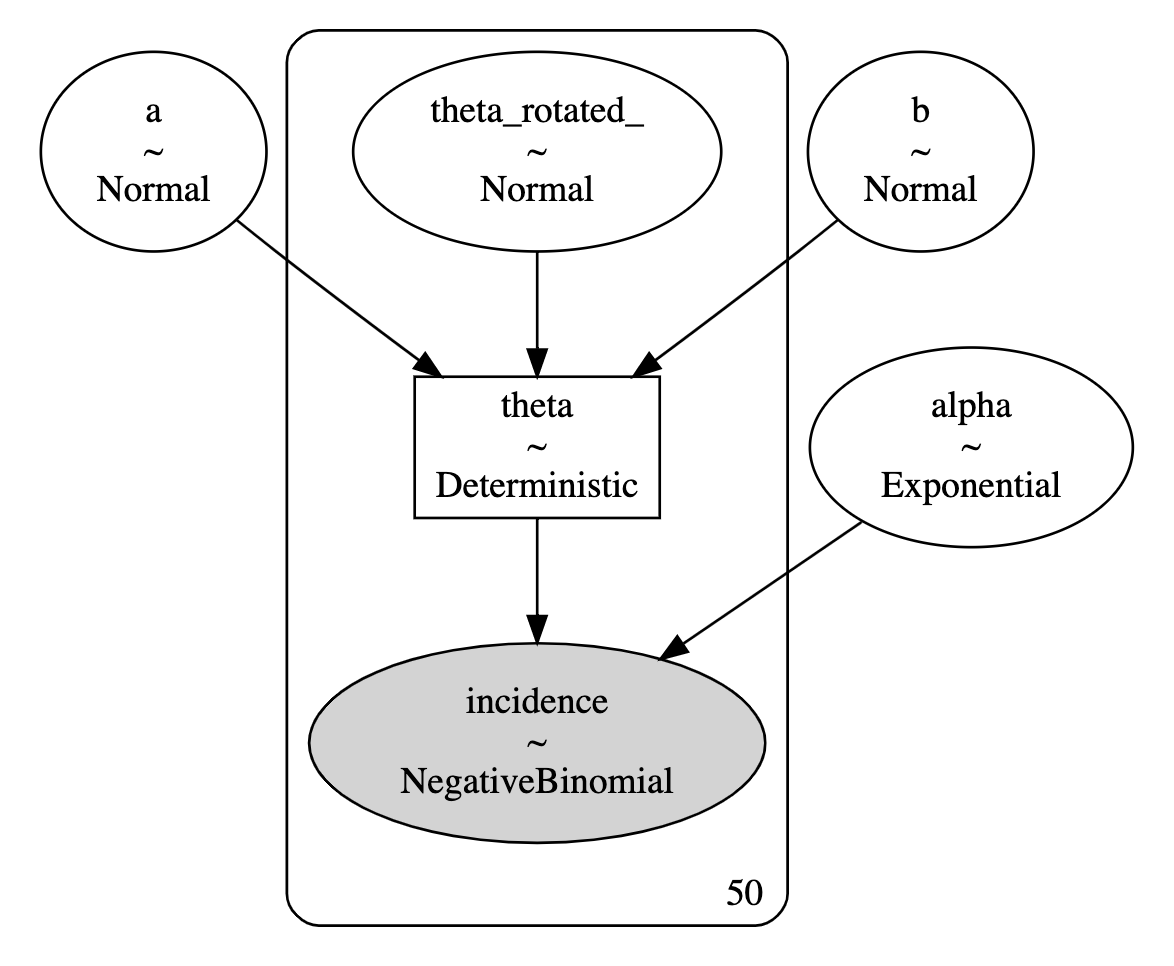
\includegraphics[width=8cm]{generated/images/inc-model-graphviz.png}
  \end{center}
  \caption{Internal PyMC3 DAG representation of our incidence model}
  \label{fig:inc-model-graphviz}
\end{figure}

To approximate incidence properly, we need to tune up model for
as much specific cases as possible. Ideally, we should try to approximate
whole incidence upon all the data, however, it will be very laborious.
Instead of that, we can grab few samples again. Those samples should
represent both regular cases and also edge cases.
For this reason, we pick the following samples for incidence validation:

\begin{enumerate}
  \item noisy incidence (\ref{fig:dev-incidence-1})
  \item low (almost zero) incidence (\ref{fig:dev-incidence-2})
  \item regular growing incidence (\ref{fig:dev-incidence-3})
\end{enumerate}

\begin{figure}[h]
  \begin{center}
    \includegraphics[width=10cm]{generated/images/theta-posterior-1.png}
  \end{center}
  \caption{Posterior of $\theta$ for sample 1}
  \label{fig:theta-posterior-1}
\end{figure}

% \begin{figure}
%   \begin{minipage}{.5\textwidth}
%     \includegraphics{images/incidence-posterior-predictive-1.png}
%    \caption{Sample 1}
%   \end{minipage}
%   \begin{minipage}{.5\textwidth}
%     \includegraphics{images/incidence-posterior-predictive-2.png}
%    \caption{Sample 2}
%   \end{minipage}
%  \end{figure}

% \begin{figure}[h]
%   \subfigure[Sample 1]{\includegraphics[width=10cm]{images/incidence-posterior-predictive-1.png}\label{fig:incidence-posterior-1}}
%   \subfigure[Sample 2]{\includegraphics[width=10cm]{images/incidence-posterior-predictive-2.png}\label{fig:incidence-posterior-2}}
%   \caption{main caption}\label{main_label}
% \end{figure}

% \begin{figure}[h]
%   \centering
%   % \begin{center}
%     \includegraphics[width=10cm]{images/incidence-posterior-predictive-1.png}
%     \caption{Posterior predictive of TODO: incidence for sample 1}
%     \label{fig:incidence-posterior-1}
%   % \end{center}

%   % \begin{center}
%     \includegraphics[width=10cm]{images/incidence-posterior-predictive-2.png}
%     % \caption{Posterior predictive of TODO: incidence for sample 2}
%     \label{fig:incidence-posterior-2}
%   % \end{center}

%   % \begin{center}
%     \includegraphics[width=10cm]{images/incidence-posterior-predictive-3.png}
%     % \caption{Posterior predictive of TODO: incidence for sample 3}
%     \label{fig:incidence-posterior-3}
%   % \end{center}
% \end{figure}

\begin{figure}[h]
  \centering
  \includegraphics[width=10cm]{generated/images/incidence-posterior-predictive-1.png}
  \caption{Posterior predictive of $\hat{c}$ for sample 1}
  \label{fig:incidence-posterior-1}
\end{figure}

\begin{figure}[h]
  \centering
  \includegraphics[width=10cm]{generated/images/incidence-posterior-predictive-2.png}
  \caption{Posterior predictive of $\hat{c}$ for sample 2}
  \label{fig:incidence-posterior-2}
\end{figure}

\begin{figure}[h]
  \centering
  \includegraphics[width=10cm]{generated/images/incidence-posterior-predictive-3.png}
  \caption{Posterior predictive of $\hat{c}$ for sample 3}
  \label{fig:incidence-posterior-3}
\end{figure}


\chapter{The risk model}

For the next steps, we will switch back to the deterministic 
world, at least, in terms of computation, to retain simplicity of our model.

\section{Prevalence estimation}

\section{Validation}

In the previous chapter, we established the probabilistic
incidence inference model capable of fit very noisy observations.
Now we have to employ previously established epimiological theory
to utilize inferred incidence to compute the risk.
In this case, the best way could be to generate artificial data
with a model of known parameters, which we can laterly try to
infer and compare.
For this purposes, we will use SIR model, which is simple 
but powerful in parametrization.
What we are going to generate is daily incidence, so recall 
the incidence equation for SIR model (TODO: discretization):

\begin{equation}
  \label{eq:risk-model-incidence}
  c = \beta_t I_{t-1} \frac{S_{t-1}}{N}
\end{equation}

The one parameter, we could compute after the inference, 
is the $\mathcal{R}_e$, therefore, we can parametrize 
the generation of artificial data with $\mathcal{R}_e$, which
is defined for SIR model as (TODO: recalling):

\begin{equation}\label{eq:risk-model-rt}
\mathcal{R}_{et} = \mathcal{R}_0 \frac{S_{t-1}}{N} = \frac{\beta_t}{\gamma_t} \frac{S_{t-1}}{N}
\end{equation}

From previous equation we can express $\beta_t$:
\begin{equation}
\beta_t = \frac{\gamma_t N \mathcal{R}_{et}}{S_{t-1}}
\end{equation}

Substituting into incidence equation \eqref{eq:risk-model-incidence} we get:
\begin{equation}
  c = \gamma_t \mathcal{R}_{et} I_{t-1}
\end{equation}

The only thing remains is to solve $\gamma_t$, this is usually given as:

\begin{equation}
  \gamma_t = \frac{1}{w}
\end{equation}

where $w$ is the mean serial interval. In our case, $w$ is a vector, therefore:

\begin{equation}
  \gamma_t = \frac{1}{\mathbb{E}[w]}
\end{equation}

\begin{figure}[h]
  \begin{center}
    \includegraphics[width=11cm]{generated/images/risk-model-fake-rt.png}
  \end{center}
  \caption{Generated $\mathcal{R}_{e}$}
  \label{fig:risk-model-fake-rt}
\end{figure}

\begin{figure}[h]
  \begin{center}
    \includegraphics[width=11cm]{generated/images/risk-model-fake-sir.png}
  \end{center}
  \caption{Generated SIR data}
  \label{fig:risk-model-fake-sir}
\end{figure}

\begin{figure}[h]
  \begin{center}
    \includegraphics[width=11cm]{generated/images/risk-model-fake-incidence.png}
  \end{center}
  \caption{Generated incidence}
  \label{fig:risk-model-fake-incidence}
\end{figure}

\begin{figure}[h]
  \begin{center}
    \includegraphics[width=11cm]{generated/images/risk-model-incidence-posterior-predictive.png}
  \end{center}
  \caption{Posterior TODO:}
  \label{fig:risk-model-fake-incidence}
\end{figure}


\chapter{Conclusion}


\cite{blei2018}





\cite{pfeffer2016}
\cite{davidson-pilon2015}


\printbibliography[heading=bibintoc]

\appendix

\chapter{An appendix}

\input{generated/tables/adf-test-brno}
\input{generated/tables/adf-test-ostrava}

\begin{figure}[H]
  \begin{center}
    \includegraphics[width=\textwidth]{generated/images/dev-incidence-1.png}
  \end{center}
  \caption{Sample 1 for the incidence inference tuning}
  \label{fig:dev-incidence-1}
\end{figure}

\begin{figure}[H]
  \begin{center}
    \includegraphics[width=\textwidth]{generated/images/dev-incidence-2.png}
  \end{center}
  \caption{Sample 2 for the incidence inference tuning}
  \label{fig:dev-incidence-2}
\end{figure}

\begin{figure}[H]
  \begin{center}
    \includegraphics[width=\textwidth]{generated/images/dev-incidence-3.png}
  \end{center}
  \caption{Sample 3 for the incidence inference tuning}
  \label{fig:dev-incidence-3}
\end{figure}


\begin{figure}[H]
  \begin{center}
    \includegraphics[width=\textwidth]{generated/images/theta-posterior-2.png}
  \end{center}
  \caption{Posterior of $\theta$ for sample 2}
  \label{fig:theta-posterior-2}
\end{figure}

\begin{figure}[H]
  \begin{center}
    \includegraphics[width=\textwidth]{generated/images/theta-posterior-3.png}
  \end{center}
  \caption{Posterior of $\theta$ for sample 3}
  \label{fig:theta-posterior-3}
\end{figure}

\newpage
\section{The source code}

\subsection{Notebook initialization}

\input{generated/snippets/init-installs.tex}
\input{generated/snippets/init-imports.tex}

\subsection{Utilities}

\input{generated/snippets/utils-base-figure}
\input{generated/snippets/utils-base-plotly}
\input{generated/snippets/utils-base-matplotlib}
\input{generated/snippets/utils-base-latex}
\input{generated/snippets/utils-adf-test}

\subsection{Data wrangling}

% \input{generated/snippets/data-serial-interval}
% \input{generated/snippets/data-serial-interval-instances}
% \input{generated/snippets/data-serial-interval-overview}
% \input{generated/snippets/data-incidence}
% \input{generated/snippets/data-largest-cities-plot}
% \input{generated/snippets/data-adf-test-prague}
% \input{generated/snippets/data-adf-test-brno-ostrava}
% \input{generated/snippets/data-seasonal-decomposition-figure}
% \input{generated/snippets/data-seasonal-decomposition-additive}
% \input{generated/snippets/data-seasonal-decomposition-multiplicative}

\end{document}
